\documentclass[11pt, letterpaper]{article}
\usepackage{amssymb,amsmath}
\usepackage{pifont}
\usepackage{graphicx}
\usepackage{txfonts}
\usepackage{natbib}
\usepackage{rotating}
\usepackage[dvipsnames]{xcolor}
\usepackage{url}
\usepackage{hyperref}
\hypersetup{
    colorlinks=true,
    linkcolor=black,
    filecolor=magenta, 
    citecolor=MidnightBlue,
    urlcolor=black,
}
% Palatino for rm and math | Helvetica for ss | Courier for tt
\usepackage{mathpazo}       % math & rm
\linespread{1.05}           % Palatino needs more leading (space between lines)
\usepackage[scaled]{helvet} % ss
\usepackage{courier}        % tt
\normalfont
\usepackage[T1]{fontenc}

%\usepackage[top=1.25in, bottom=1.25in, outer=1.25in, inner=1.25in, heightrounded, marginparwidth=1.0in, marginparsep=0.25in]{geometry}
\usepackage[margin=1.00in]{geometry}    % Leave a one-inch margin around all text.
% If a conflict exists between template and instructions: follow the instructions document!

\usepackage{setspace} % Needed for doublespacing
\graphicspath{ {../Figures/} }
\usepackage{pdflscape} % Needed for landscape table

% abbreviations used in this paper
% Define local notation.

\def\etal{{\emph{et alia\/}}}
\def\sR{\textsf{R}}
\def\argmax{\mathop{\rm argmax}}
\def\cL{{\cal L}}


\begin{document}
\doublespacing % Your outline should be printed double-spaced on 8.5x11-inch paper. 

\title{Selecting the Optimal Credit Card Portfolio\\
       Project Outline\\
       {\large ECO 6935 -- Capstone in Business Analytics I}}
%      {\large ECO 6935}\\
%      {\large Capstone in Business Analytics I}}
\author{Remco A.~Scheepmaker}
%\date{xx July 2024}
\date{\today}

\maketitle

% \begin{abstract}
% 


% \bigskip
% \bigskip

% \noindent
% \textbf{Keywords:} one; two; three.

% \bigskip

% \noindent
% \textbf{JEL Classification Numbers:} C57, C61, C72.
% \end{abstract}

% \vfill
% \eject

\section{Introduction} \label{sec:Introduction}
% OUTLINE: 
% Your outline should have the following structure: In the first section, provide a brief description of your topic, including some institutional information that will make possible an evaluation of the theoretical model you have chosen, to be presented in a later section. 

% FINAL PAPER:
% an introduction, where the problem is motivated and the interesting features of the analysis summarized;

Credit cards are an important part of the American economy and culture.
According to the Consumer Financial Protection Bureau \citep{cfpb:2023}, consumers spent \$3.2 trillion on purchases using credit cards in 2022. 
Total credit card debt recently passed \$1 trillion, 82 percent of which is revolving (i.e. bearing interest, the remaining 18 percent is paid by the due date without being charged interest). 
The combination of income from interest, interchange fees, and annual fees makes credit cards very profitable for the major banks, but they can also be profitable for a certain fraction of their users.
A key feature of many credit cards is their rewards structure, which returns a percentage of the user's spend back to the user in the form of cash back, reward points, or miles.%
\footnote{I consider points and miles to be the same for this project. Both can generally be redeemed for cash, statement credit, or used to book travel, either by transfering to loyalty programs of travel partners, or by booking flights and hotels directly through the bank's own travel portal.}
Credit card rewards programs are designed by banks to attract new customers and improve their loyalty, as well as to increase income through interchange fees and interest by stimulating (over)spending.
The CFPB estimates that the total dollar value of the rewards earned in 2022 exceeded \$40 billion, and the average rewards-earning account redeemed \$167.%
\footnote{According to Experian, the average American has 3.9 credit card accounts (\url{https://www.experian.com/blogs/ask-experian/average-number-of-credit-cards-a-person-has/}, accessed June 1, 2024).} 
These ``earnings'' are much less than the \$130 billion charged to consumers in interest and fees, making credit cards such a profitable enterprise for banks. 

As we will see in more detail in the next section, credit card rewards work partially through what is called the ``reverse Robin Hood'' mechanism, since to some extend it is the poor who, by paying interest and fees, subsidize the rewards of the rich \citep{wsj:2010}.
%\footnote{\url{https://www.wsj.com/articles/BL-REB-11033}}
More accurately, it is primarily the financially na\"{i}ve who are sponsoring the financially sophisticated, where the level of sophistication seems best measured by credit scores from the Fair Isaac Corporation (FICO), as opposed to income \citep*{agaretal:2023}.
%(Agarwal, Presbitero, Silva, and Wix, \citeyear{agaretal:2023}).
For those interested in travel using credit card points, or just saving some money through cashback rewards, it is therefore crucial to learn good financial habits and eventually become part of the financially sophisticated demographic with high FICO scores. 

Once credit card rewards are a net benefit (meaning the value of the rewards are higher than the costs of fees and interest), it might be worthwile to explore how we can optimize one's choice of credit cards to maximize this benefit. Which credit cards should different consumers select, and is there an optimal number before the marginal benefit of adding more cards becomes too small?  
These are the topics I study in this project. 
My personal credit card portfolio has expanded from two to eleven credit cards over the last five years, increasing my net benefit from less than two to about five percent of my entire annual spend.
The analysis that I applied to my own spending budget, in order to optimize my own credit card portfolio, inspired me to create an optimization algorithm that can be applied at scale to a larger selection of credit cards, and to different types of consumers. 
In this paper I present this algorithm, code it in \sR, and use it to model ``optimal'' portfolios of rewards credit cards for various combinations of user preferences and spending characteristics. 
I then study the properties of these modeled portfolios by combining data from the Bureau of Labor Statistics (BLS) on income and spending with data on credit card reward multipliers and values. 
By performing a sensitivity analysis, I find that spending on four to six credit cards is the sweet spot for most people, before the marginal benefit of adding more cards to the portfolio drops below \$50. 
From a Monte Carlo simulation I find that the average return on spend (ROS) is 3.8~percent, with a standard deviation of 0.8~percent. 
In terms of ROS, the benefit of using credit cards can be significantly higher (up to $\sim$6.5~percent) for people who do not spend a lot but make full use of static benefits, such as travel credits and airport lounge access, or for people who spend above average on travel, since the travel categories have the highest (uncapped) point multipliers. 
Finally, I present a \textsf{Shiny} app that I developed in \sR, to serve as an online tool that people can use to get a recommended credit card portfolio, based on their personal preferences and spending budget.
This app can benefit many sophisticated credit card users who would like to stretch their budgets, travel more, or who simply enjoy optimizing their personal finances.

The structure of this paper is as follows. 
In Sect.~\ref{sec:Literature}, I first discuss some literature and background on credit scores and the payment structure of rewards programs. 
In Sect.~\ref{sec:Theory}, the theoretical model that will form the basis of my optimization algorithm is presented. 
In Sect.~\ref{sec:Specification}, the theory is broken down into an empirical specification that depends on variables and parameters that will need to come from data.
In Sect.~\ref{sec:Data}, the sources for these data are described. 
In Sect.~\ref{sec:Results}, I present the results, which includes the sensitivity analysis and Monte Carlo modeling, as well as a description of the \sR\ \textsf{Shiny} app that has also been deployed online. 
Finally, the conclusions are discussed in Sect.~\ref{sec:Conclusions}, and the appendices are reserved for some tables that show additional details of the data, as well as the code that makes up the recommendation algorithm.

% Your outline should have the following structure: In the first section, provide a brief description of your topic, including some institutional information that will make possible an evaluation of the theoretical model you have chosen, to be presented in a later section. 

\section{Literature} \label{sec:Literature}
% In the next section, present a summary of what other authors have written on your topic.

The latest ``Consumer Credit Card Market'' report from the \citet{cfpb:2023} contains a wealth of information about how Americans use their credit cards, separated by FICO credit scores according to the levels shown in Table~\ref{tab:FICO}.
The CFPB reports that more than 90 percent of the purchase volume is on rewards cards, and that the average rewards-earning account contained \$156 in 2022. 
But, as we can see in Fig.~\ref{fig:CFPBRewardsBalances}, accounts with high credit scores have considerably higher rewards balances compared to accounts with low credit scores. 
The CFPB also finds that people with prime plus or superprime credit scores keep zero, or very low, revolving balances, while their purchase volumes and payment rates are actually the highest. 
This is consistent with practicing good financial habits in order to enjoy the benefits of credit card rewards and reach a high FICO score.%
\footnote{Although the exact algorithm is proprietary, there are many online resources that explain what a FICO score consists of, and how one can improve it, e.g. \url{https://www.myfico.com/credit-education/credit-scores}.}
The most important habit regarding rewards is to pay off statement balances \emph{in full} by the due date each month (so no interest on revolving balances is paid). This implies only using credit cards for purchases that you can afford to pay off completely the next month.

% Table of FICO thresholds according to the CFPB and Agarwal et al. (2023)    
\begin{table}[t!]
    \centering
    \begin{tabular}{ r c c } 
        \hline
        & CFPB & Agarwal \emph{et al.} (2023) \\ 
        \hline
        deep sub-prime & $<580$ & \\
        sub-prime & 580--619 & $<660$ \\ 
        near-prime & 620--659  & 660--719 \\ 
        prime & 660--719 & 720--779 \\ 
        prime plus & 720--799 & \\
        super-prime & $>799$ & $>779$ \\ 
        \hline
    \end{tabular}
    \caption{FICO score thresholds used by the CFPB and \citet{agaretal:2023}.}
    \label{tab:FICO}
\end{table}


\begin{figure}[t!h]
    \begin{center}
    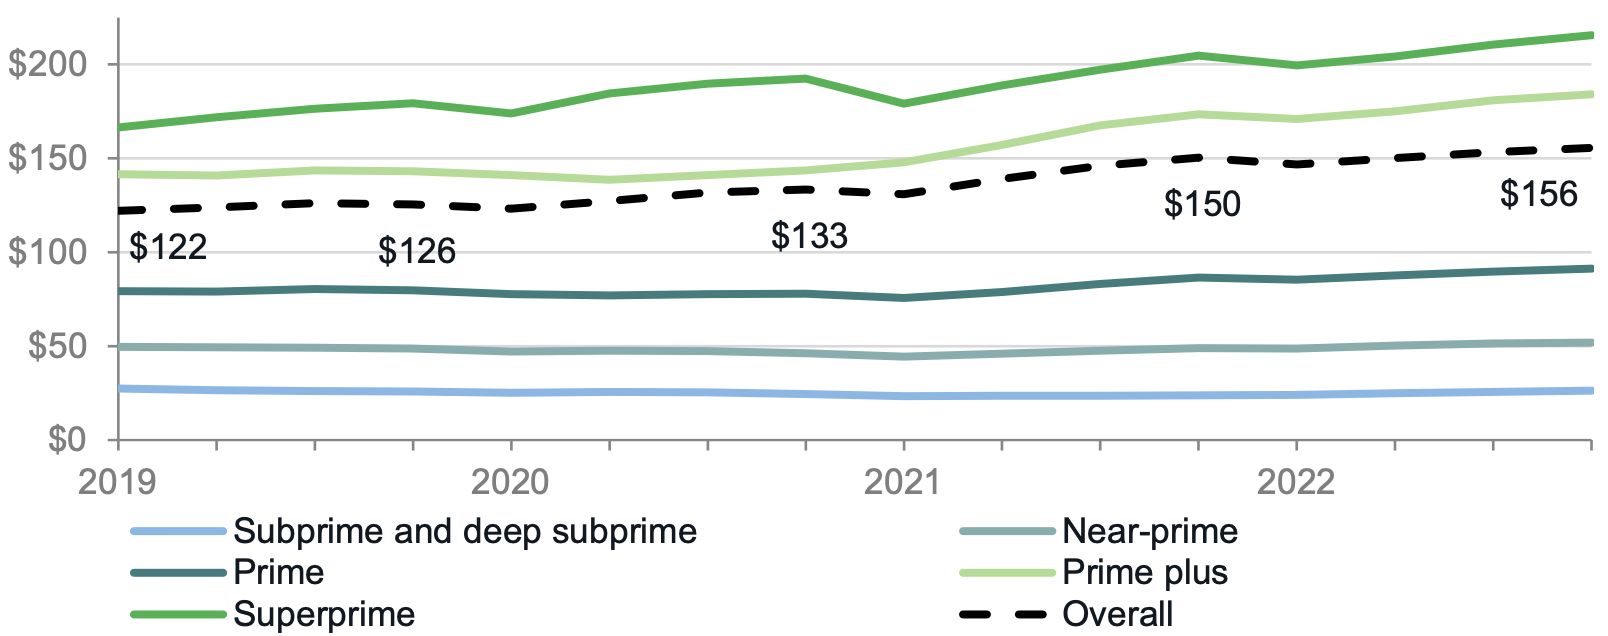
\includegraphics[width=0.8\textwidth]{../Misc/CFPBFig2_DollarPerAccount.png}
    \caption{Quarterly dollar value of average rewards balances for different credit scores. Source:~\citet{cfpb:2023}.}
    \label{fig:CFPBRewardsBalances}
    \end{center}
\end{figure}

While it is true that applying for new credit cards results in the banks ``pulling'' the applicant's credit report, lowering the credit score, it is important to note that this effect is only temporary. In the long run, opening many credit cards to optimize rewards can actually have a positive impact on credit scores, as the ``utilization ratio'' per card is lowered (the amount of spending on the card as a percentage of the credit limit). 
As an example, Fig.~\ref{fig:FICOTimeline} shows a time series of my personal credit scores with the dates of nine credit card applications marked. Even with this above-average number of credit card applications, the overall trend in credit scores is positive.

\begin{figure}[t!h]
    \begin{center}
    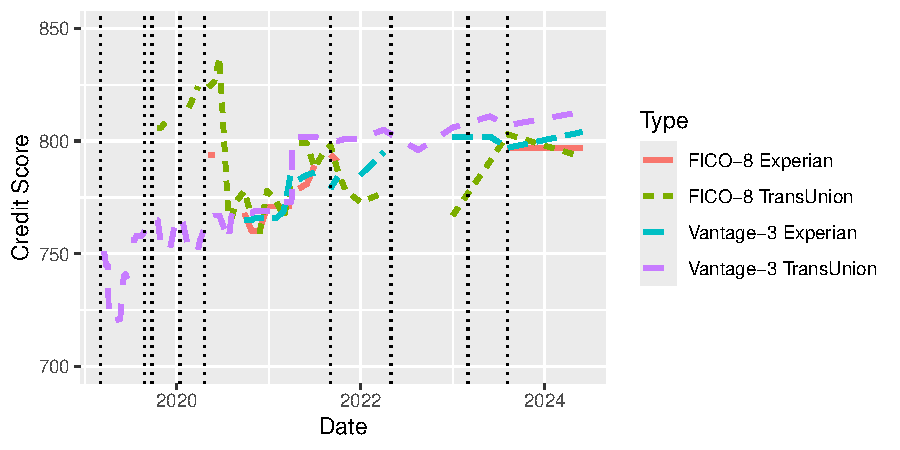
\includegraphics[width=1.0\textwidth]{CreditScoresTimeSeries.pdf}
    \caption{Time series of my personal credit scores. The vertical dotted lines mark the dates when new credit card accounts were opened.}
    \label{fig:FICOTimeline}
    \end{center}
\end{figure}

Regarding the payment structure of rewards programs, Fumiko Hayashi \citeyearpar{hayashi:2009} shows a good overview of the payment fee flows between the merchant, the merchant acquirer (the bank that processes card payments for the merchant), the card issuer (the cardholder's bank) and the cardholder.
In an example where the cardholder makes a \$100 purchase, the merchant receives \$97.50. The \$2.50 in fees is split between the merchant acquirer (\$0.50) and an interchange fee of \$2.00 that is paid from the merchant acquirer to the card issuer. The card issuer pays a fraction of the interchange fee (say \$1.00) as a reward to the cardholder, and also pays the card network (such as Visa or MasterCard), who set the interchange fees.%
\footnote{American Express transactions work differently, as American Express operates its own network and simultaneously acts as both card issuer and merchant acquirer.}
The merchant is likely to pass on these fees as higher retail prices to the consumer (regardless of the payment method). \citet{hayashi:2009} concludes that it is not completely clear who ultimately pays for the rewards programs, but it seems likely that credit card rewards programs are not efficient markets. 
For rewards programs to be Pareto efficient, the use of credit cards would have to lead to cost savings for the merchants (due to less handling of cash, which comes with security risks and depositing costs). 
Only the savings beyond the operating costs of handling credit card transactions would then be returned to customers in the form of rewards, in which case everyone is better off without anyone being worse off. Such a scenario seems unlikely, as many merchants complain about interchange fees being too high. 

\begin{figure}[t!h]
    \begin{center}
    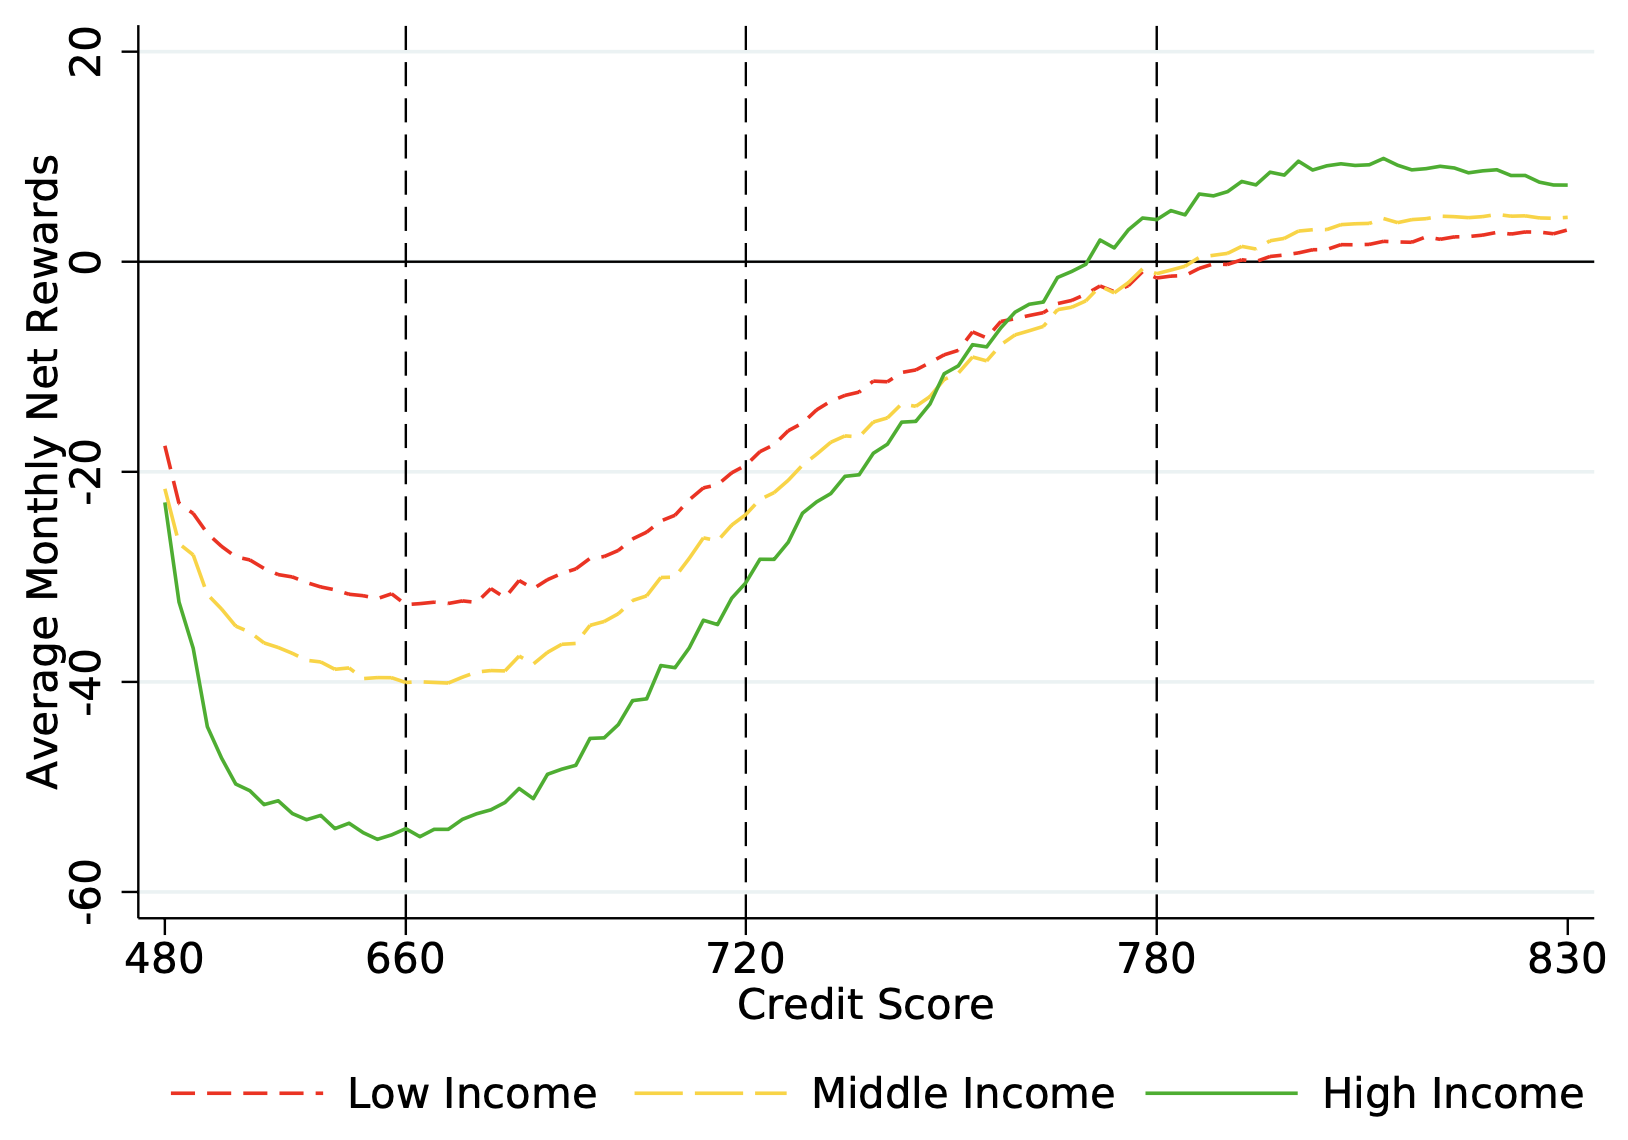
\includegraphics[width=0.7\textwidth]{../Misc/Agarwal_NetRewardsByIncome.png}
    \caption{Average monthly net rewards by income and credit score. Source: \citet{agaretal:2023}.}
    \label{fig:AgarwalRewards}
    \end{center}
\end{figure}

\citet*{schuetal:2010} find that it is cash-using households who are paying for the rewards of card-using households, which, due to the positive correlation between income and use of credit cards, translates to lower incomes paying for the rewards of higher incomes (the ``reverse Robin Hood'' mechanism). 
However, \citet*{agaretal:2023} show that this redistribution takes place from low to high FICO scores \emph{regardless} of income.
As Fig.~\ref{fig:AgarwalRewards} shows, it is primarily the super prime cardholders who have positive monthly net rewards, while the sub-prime and near-prime cardholders pay the most for using rewards cards. Interestingly, high-income, super-prime cardholders benefit the most (\$20.1 in net rewards per month), primarily at the expense of \emph{high-income} cardholders with low credit scores.

\citet*{agaretal:2023} use FICO scores as a proxy for financial sophistication, and conclude that ``sophisticated individuals profit from reward credit cards at the expense of na\"{i}ve customers.''
They also estimate the aggregate annual redistribution to be \$15 billion and find that this redistribution takes place from less to more educated, poorer to richer, and high to low minority areas, widening existing disparities.

% Even though in this project I do not have access to detailed data on people's income, zip codes, and credit card usage, it will be interesting to compare some of these results to a modeling exercise that accounts for different types of credit card users. 

% https://fredblog.stlouisfed.org/2023/10/credit-card-holders-and-their-credit-scores/ 

% In the next section, present a summary of what other authors have written on your topic.

\section{Theoretical Model} \label{sec:Theory}
% In the third section, present your theoretical model, pointing out the implications of the model for the business problem you are trying to solve. 

Above we have seen that, in order to maximize the net benefits of credit card rewards, 
we should show ``sophisticated'' financial behavior.
Assuming we have such a sophisticated credit card user who never pays interest, and who spends her entire discretionary budget (staying within her means) using rewards credit cards, I will model the maximum net benefit for a different number of credit cards and for different types of users (e.g. users who will redeem credit card points for travel versus users who are only interested in cashback).

All reward credit cards come with certain point multipliers in specific categories, that will be multiplied with the spend in that category to calculate the number of points. 
For cashback rewards, the value of a point is per definition one cent, but for certain cards the value of a point can vary between a lower value (base value) and a higher value when redeemed for travel. 
Cards might also have an annual fee, or come with certain static benefits such as airport lounge access, travel or food credits, and discounts toward certain subscriptions such as Disney$^{+}$. 
In this project I will ignore sign-up bonuses (SUBs), which were 9.1 percent of total reward earnings in 2022 \citep{cfpb:2023}, since these high (but one-time) SUBs will always result in a very high marginal benefit for relatively little spend. Including them would  lead to the conclusion that it is always beneficial to open another account with a SUB, into perpetuity.%
\footnote{People who keep opening new credit card accounts just for the SUB are known as \emph{churners}.}  
%SUBs are higher for below-prime scores, CFPB page 104).

The problem of optimizing a credit card portfolio comes down to maximizing the net benefit by selecting, say at most, $K$ credit cards from a dataset of $N$ possible cards.
By itself, an algorithm to solve such a problem would, at best, need exponential-time resources, and is therefore NP-hard and intractable \citep*[][Sect.~6.2.3]{paargoly:2016}.
Luckily for us, people usually apply for credit cards one at a time, and over the course of months or years. 
We can therefore easily discipline our problem by assuming that people start with a single credit card, and subsequently add cards to their portfolio.
Smaller portfolios are also preferred for the sake of simplicity (and limited wallet space).
This additional structure turns our problem of selecting the optimal credit card portfolio into a tractable \emph{greedy} algorithm: the problem is broken down into smaller subproblems (``what is the best card to add now?''), and the best solution (highest additional value) is selected first.
It also uses elements from \emph{dynamic programming}, since we will need to store the intermediate solutions, and we will be using tables to calculate the marginal benefit that can still be extracted from the remaining cards.

The first subproblem is to the select the best single card, and use it for all our spending categories. 
For adding an additional card, we have to consider all remaining cards and compare the value for each spending category to the previous card that we had already selected.%
\footnote{In code, I implemented this by creating a matrix with the values per card and spending category. The values of the previously selected card are subtracted from this matrix, and negative values are set to zero. The remaining positive values show where additional value can be extracted from the corpus of cards.} 
The card with the highest additional net benefit (summing all categories and benefits, and subtracting fees) is added to the portfolio, and a table with the best card to use for each category is updated. 
To select $K$ cards, we have to repeat the search through all $N$ possible cards $K$ times, making this a feasible algorithm with complexity $\mathcal{O}(N)$.
%C categories, N card corpus size, K cards selected.

% In the third section, present your theoretical model, pointing out the implications of the model for the business problem you are trying to solve. 

\section{Empirical Specification} \label{sec:Specification}
% From your theoretical model, then develop an empirical specification within which you can provide a business or economic or behavioral interpretation in the fourth section. 

The theoretical model described in Sect.~\ref{sec:Theory} can be broken down into the following empirical specification. For every credit card $k$ we have for the value earned per spending category $c$:
%
\begin{equation}
    y_{kc} = x_{kc}\/m_{kc} \left[ \eta\/ v_{t,k} + 
    (1 - \eta)\/ v_{b,k}\right],
\end{equation}
%
where $x_{kc}$ is the spend on card $k$ in category $c$, $m_{kc}$ is the card multiplier for that category, $v_{t,k}$ and $v_{b,k}$ are the card's highest and lowest point redemption values, and $\eta$ quantifies which fraction of the points are used for the higher-valued travel redemptions (a user-specific variable). The total value from spending is simply found by summing over the $C$ possible categories:
%
\begin{equation}
    s_{k} = \sum_{c=1}^{C}y_{kc}.
\end{equation}
%
For the total benefit we add the static benefits $b_{k}$ multiplied with the fraction of their use $\theta$, subtract the annual fees $f_{k}$, and sum over all the $K$ cards in our portfolio:
%
\begin{equation} \label{eq:specification}
    Y(\mathbf{X}, K, \eta, \theta | \mathbf{M}, \mathbf{v_{t}}, \mathbf{v_{b}}, \mathbf{b}, \mathbf{f} ) = \sum_{k=1}^{K}\left( s_{k} + \theta\/ b_{k} - f_{k}\right).
\end{equation}
%
Here it is made explicit that the total benefit $Y$ depends on user-specific variables $\mathbf{X}$ (the budget matrix with spending per card and category), $K$ (the number of cards), $\eta$ (the fraction of travel redemptions), and $\theta$ (the fraction of benefits used), and the card-specific parameters $\mathbf{M}$ (a matrix with the multipliers per card and category), $\mathbf{v_{t}}$ (a vector with travel point values), $\mathbf{v_{b}}$ (a vector with base values), $\mathbf{b}$ (a vector with benefits), and $\mathbf{f}$ (a vector with annual fees).
One of the goals of this project is to study $Y$ as a function of its variables, given the parameters.
The other goal is to return the list of credit cards (including a list of which card to use for which category) that maximizes $Y$, after a user inputs the variables $\mathbf{X}, K, \eta$, and $\theta$.
% From your theoretical model, then develop an empirical specification within which you can provide a business or economic or behavioral interpretation in the fourth section. 

\section{Data} \label{sec:Data}

The empirical specification from Sect.~\ref{sec:Specification} (Eq.~\ref{eq:specification}) implies that we need data on rewards credit cards point multipliers, point values, benefits, and fees, as well as budget data for our credit card users.

\subsection{Credit Card Data} \label{subsec:CreditCardData}

There are many websites writing about rewards credit cards, their perks, and points structure. 
I mainly used the website allcards.com%
\footnote{\url{https://www.allcards.com} (accessed between June 3--9, 2024).}
to manually scrape the information on point multipliers and their caps (limits) from the most popular rewards credit cards from the seven major banks (American Express, Chase, Bank of America, Citi, Capital One, US Bank, and Wells Fargo). 
The bank websites were used to find some missing information, if needed. 
This resulted in a list of 28 unique credit cards. 
However, some of the cards have a ``custom'' bonus reward category that can be chosen by the user (e.g. 5x points on groceries, or gas, or home improvement up to \$6000 per year). 
These cards were treated as a separate credit card for each bonus category, bringing our total number of cards to 38. 

I ignored credit cards that are dedicated to users of very specific stores, hotels, or airlines, as well as cards with rather exotic, or variable, reward categories (such as ``3x points on all mobile wallet payments'', or ``5x points on quarterly changing categories''), since these categories are impossible to map to our budget categories that will be discussed in the next section. 
The results on total benefits should therefore be considered \emph{lower limits}, as there are many cards that can bring additional benefits to loyal users of certain brands.
 
A list of 18 common card spending categories was taken from the website cardpointers.com,%
\footnote{\url{https://www.cardpointers.com/app/} (accessed between June 3--9, 2024).}
with the modification of removing ``warehouse clubs'' and ``ride sharing'', and adding ``streaming'' and ``travel (other)'', to facilitate a mapping of all the items on our budget to a spending category (see Sect.~\ref{subsec:UserData}). The final list of all the categories can be found in the first column of Table~\ref{tab:BudgetExtended} in the Data Appendix.

For the base and travel values of the credit card points, I used the table from the \citet{nerdwallet:2024} website. 
These values are shown in Table~\ref{tab:PointValues} in the Data Appendix and will be used for the sensitivity analysis and Monte Carlo simulation.
Point values can be subjective, however, so for the \sR\ \textsf{Shiny} recommendation app, I foresee an update in the near future, making the point values adjustable by the user. 

Annual fees were also collected for all the cards in the dataset, as well as an estimate for the static benefits. 
We refer the reader to the Data Appendix on page~\pageref{app:Data} for a more detailed description of how the static benefits were handled. 
The appendix also shows an exerpt of the final credit card dataset in Fig.~\ref{fig:CreditCardsCSV}.


\subsection{User Data} \label{subsec:UserData}

For our credit card users we need a vector $\mathbf{x}$ with the amount of spend for each of the 18 spending categories. 
In the credit card portfolio recommendation app, the user can specify a personal yearly budget. 
For our analysis of how the optimal portfolios behave for different user preferences and budgets, however, we need realistic estimates of the average spending of Americans, since regulations and privacy concerns make obtaining actual spending data practically impossible for researchers outside of the banking sector.
I will therefore use the 2022 Consumer Expenditure Survey (CES) from the Bureau of Labor Statistics \citep{bls:2023}.

According to the CES, the average annual expenditures in 2022 were \$72,967 (after savings), from an average income before taxes of \$94,003.
To approximate the amount that can be spend on credit cards, I subtracted from the \$72,967 the expenses on shelter (such as mortgage, rent, property taxes), vehicle purchases, health insurance, education, cash contributions, personal insurance, and pensions.
The resulting budget totals to \$38,576 or 41 percent of the average gross income. 
The remaining CES items were then mapped to the credit card spending categories according to Table~\ref{tab:BudgetExtended} in the Data Appendix. Note that some items were split 50/50 over multiple credit card categories, to make sure that all the categories were populated with some reasonable spend. For example, I assumed that the CES item ``Apparel and services'' is split 50/50 between the ``Online shopping'' and ``Department store'' credit card categories. 

The CES also provides expenditures separated by nine income levels. 
I have repeated the above construction of the average budget also for these nine income bins separately, and saved the results in the file \texttt{BudgetIncome.csv}. The percentages spend per credit card category are also shown in Table~\ref{tab:BudgetIncome} in the Data Appendix.
For a given user's income (before taxes), the corresponding income bin from this table is used to calculate the average budget, namely by multiplying the gross income by the percentage spend in each category. 
Our algorithm will then predict the total credit cards benefit as a function of income, as well as $\eta$, $\theta$, and the number of credit cards $K$ (see Sect.~\ref{sec:Specification}). 

\begin{figure}[t!h]
    \begin{center}
    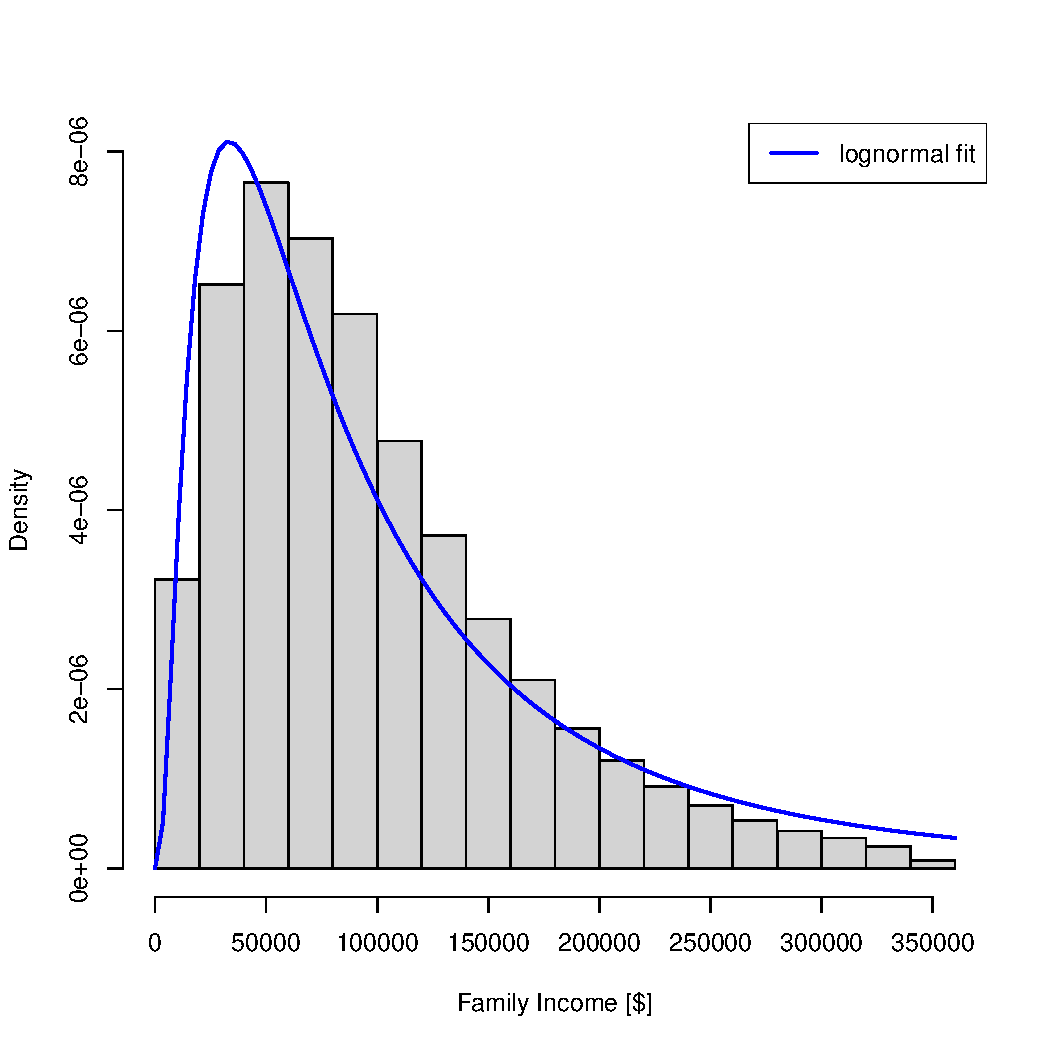
\includegraphics[width=0.6\textwidth]{../Figures/IncomeDistribution.pdf}
    \caption{2022 Florida income distribution from the BLS ACS (microdata sample of 57,005 observations, truncated at \$350,000 for this visualization).}
    \label{fig:IncomeDistribution}
    \end{center}
\end{figure}

A Monte Carlo simulation should give a reasonable estimate of the average net benefit and standard deviation for Americans who use an optimized credit card portfolio. 
For this simulation we need to sample (with replacement) income, $\eta$, $\theta$, and $K$ from realistic distributions. 
For the income distribution I used 2022 ``Family income'' (variable FINCP) from the BLS American Community Survey (ACS) Microdata tables, selecting all counties in Florida (resulting in 57,005 individual incomes).%
\footnote{\url{https://data.census.gov/mdat/\#/search?ds=ACSPUMS1Y2022} (accessed June 25,2024).}
This income distribution is shown in Fig.~\ref{fig:IncomeDistribution} and approximates a lognormal distribution.
User preferences $\eta$ and $\theta$ are sampled from a uniform distribution between 0--1, and $K$ is sampled from a uniform distribution between 1--8.

% In the fifth section, describe the sources from which you intend to draw the data necessary in training the empirical specification. 
% This will involve a complete description of each variable you intend to use from each source as well as a listing of the formulae you intend to use in transforming these variables into measures which are germane to your 

% \section{Results}   \label{sec:Results}

In this section, I first present the algorithm I developed to return the optimal credit card portfolio, given a set of user variables and card parameters.
I then describe the results of a sensitivity analysis and Monte Carlo simulation that show how the return on spend and marginal benefit depend on the user variables.
Finally, I will describe the interactive \sR\ \textsf{Shiny} app that is available online for people to play with, and to get a recommended credit card portfolio tailored to their personal preferences. 

\subsection{Portfolio Recommendation Algorithm}

The model described in Sections \ref{sec:Theory} and \ref{sec:Specification} is coded in \sR\ using two functions that are saved in the file \texttt{CCPortfolioFunctions.R}.
The function \texttt{get\_budget(income, budget\_data)} is a helper function that returns the budget as a named vector, given a gross income, corresponding to the 18 credit card categories from Sect.~\ref{subsec:CreditCardData} and using the BLS CES income-dependent data described in Sect.~\ref{subsec:UserData}.
This budget is then used as input for the second function, \texttt{get\_portfolio(K, eta, theta, cards\_data, budget, verbose = TRUE)}, which returns a named list with the optimized portfolio of credit cards, as well as some other useful metrics (the total net benefit in dollars, percentage return on spend, the marginal benefit in dollars per card, the total spend, and which card to use for each spending category). 
The full code of both these functions is presented in the Code Appendix on page~\pageref{app:Code}. 

\begin{figure}[tbh]
    \begin{center}
    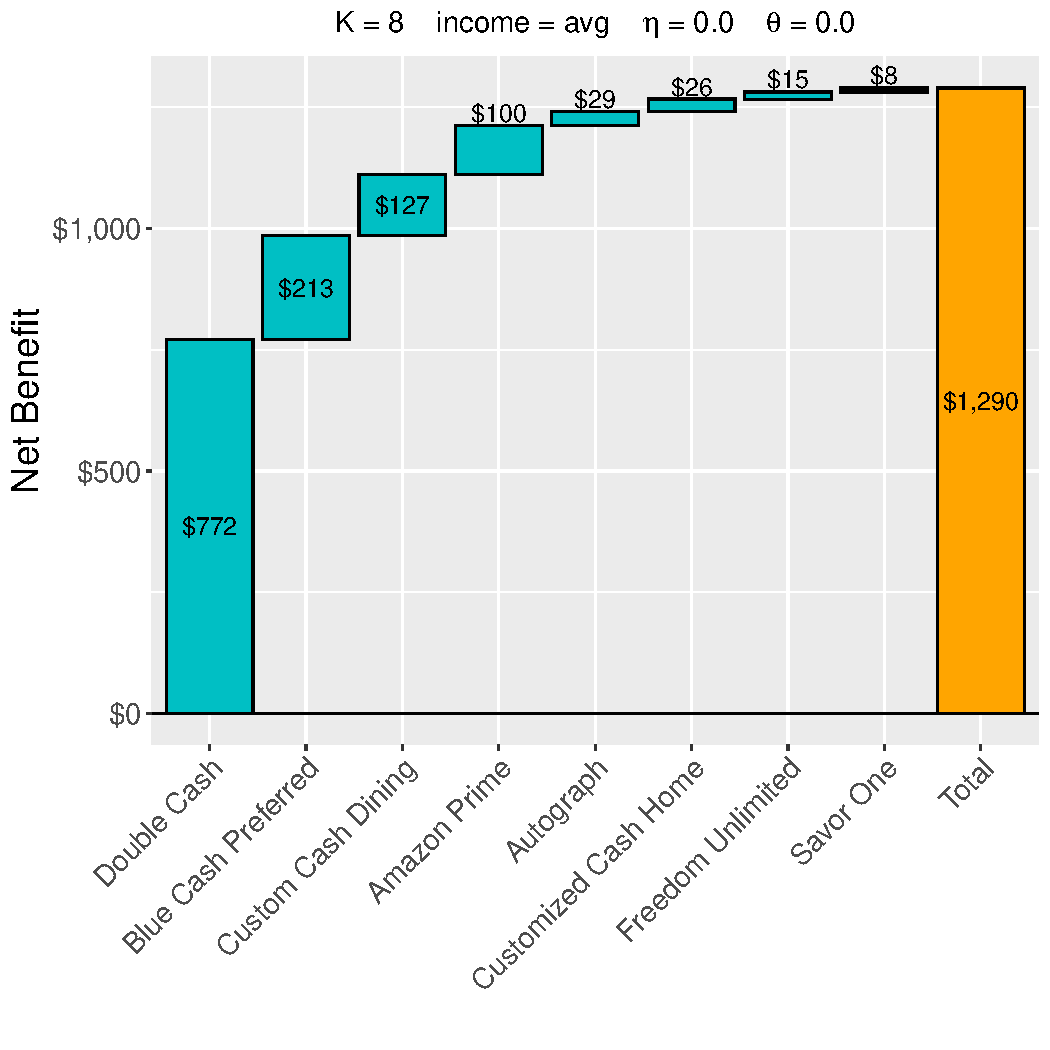
\includegraphics[width=0.6\textwidth]{../Figures/Waterfall_avg_8_0_0.pdf}
    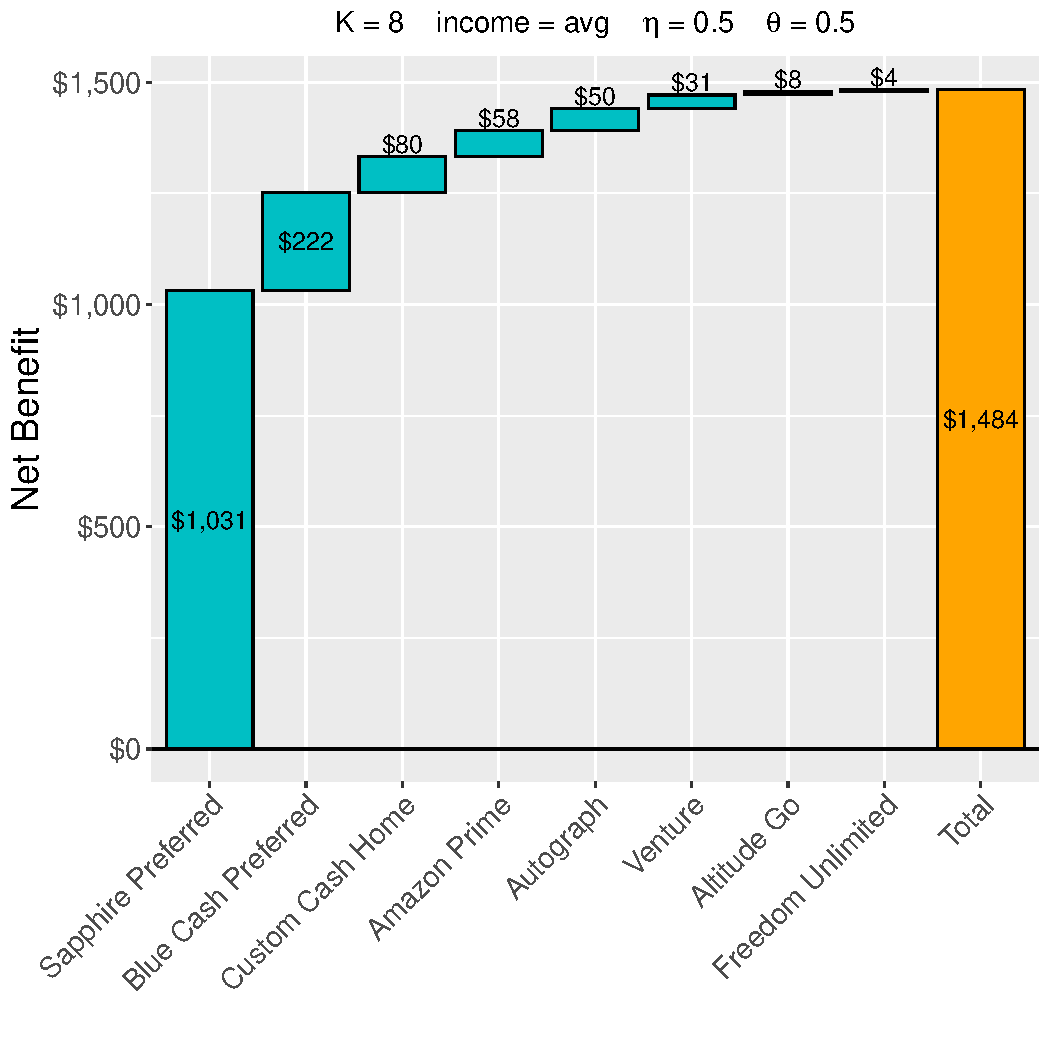
\includegraphics[width=0.6\textwidth]{../Figures/Waterfall_avg_8_05_05.pdf}
    \caption{Waterfall-style summary of two recommended portfolios, for different user preferences. Both figures returned the best 8 cards ($K=8$) for the budget of the average consumer (income $=$ avg). The first card is on the left, and the bars indicate the marginal benefit of adding each additional card. The user in the top panel has a cashback preference, and uses no static benefits ($\eta$ and $\theta$ both equal 0). The user in the bottom panel transfers half the points to travel partners ($\eta = 0.5$) and uses half of each card's benefits ($\theta = 0.5$).}
    \label{fig:Waterfall}
    \end{center}
\end{figure}

Figure~\ref{fig:Waterfall} summarizes some of the algorithm's essential output in a user-friendly format, for two different user preferences. 
The figure shows that the algorithm is successful in recommending different portfolios for different users. 
The more cashback-oriented user (top panel) gets recommended more cashback focused cards, while the more travel-oriented user (bottom panel) gets recommended a few more travel focused cards, which results in a higher total benefit (the orange bar on the right).
Note that the marginal benefit plotted per card is the \emph{additional} benefit that the card delivers, \emph{on top} of the cards already selected to its left.  
In other words, this marginal benefit includes the opportunity cost of taking spend categories away from the cards to its left, in order to put that spend on the additional card. 

Figure~\ref{fig:Waterfall} also shows that the marginal benefit diminishes with more cards, which is by design of the greedy algorithm. 
The algorithm will always recommend cards with the highest marginal benefit first. 
It is up to the user of the recommendation app (see Sect.~\ref{subsec:ShinyApp}) to decide at which marginal benefit it is no longer worth it to add additional cards, but for the remainder of this paper I assume that \$50 is probably a reasonable amount for most people to stop adding to the portfolio. 
This allows me to determine the ``sweet spot'' for the credit card portfolio size, as a function of the variables. 
I discuss this sweet spot, along with some other metrics of the recommended portfolios, in the next section.

\clearpage
\subsection{Sensitivity Analysis}

Figures \ref{fig:MBvsKvsIncome_0_0}, \ref{fig:MBvsKvsIncome_05_05}, and \ref{fig:MBvsKvsIncome_1_1} show the marginal benefit as a function of the number of cards, for different incomes, and for $(\eta, \theta)$ equal to $(0,0)$, $(0.5,0.5)$, and $(1,1)$, respectively.
The income levels for these figures are chosen to represent the average incomes of the nine income levels of the BLS CES data (Table~\ref{tab:BudgetIncome} in the Data Appendix), while the thick black dashed line represents the average budget of all consumers in the survey (with an average income of \$94k).
These figures show that for most people, regardless of preferences or income, four or five is the sweet spot for the number of credit cards to hold, before the additional benefit drops below \$50.  
There seems to be some evidence that the highest three income levels (above $\$100,000$) maintain a higher marginal benefit with more cards (up to six or seven, before the benefit drops below \$50).

\begin{figure}[tbh]
    \begin{center}
    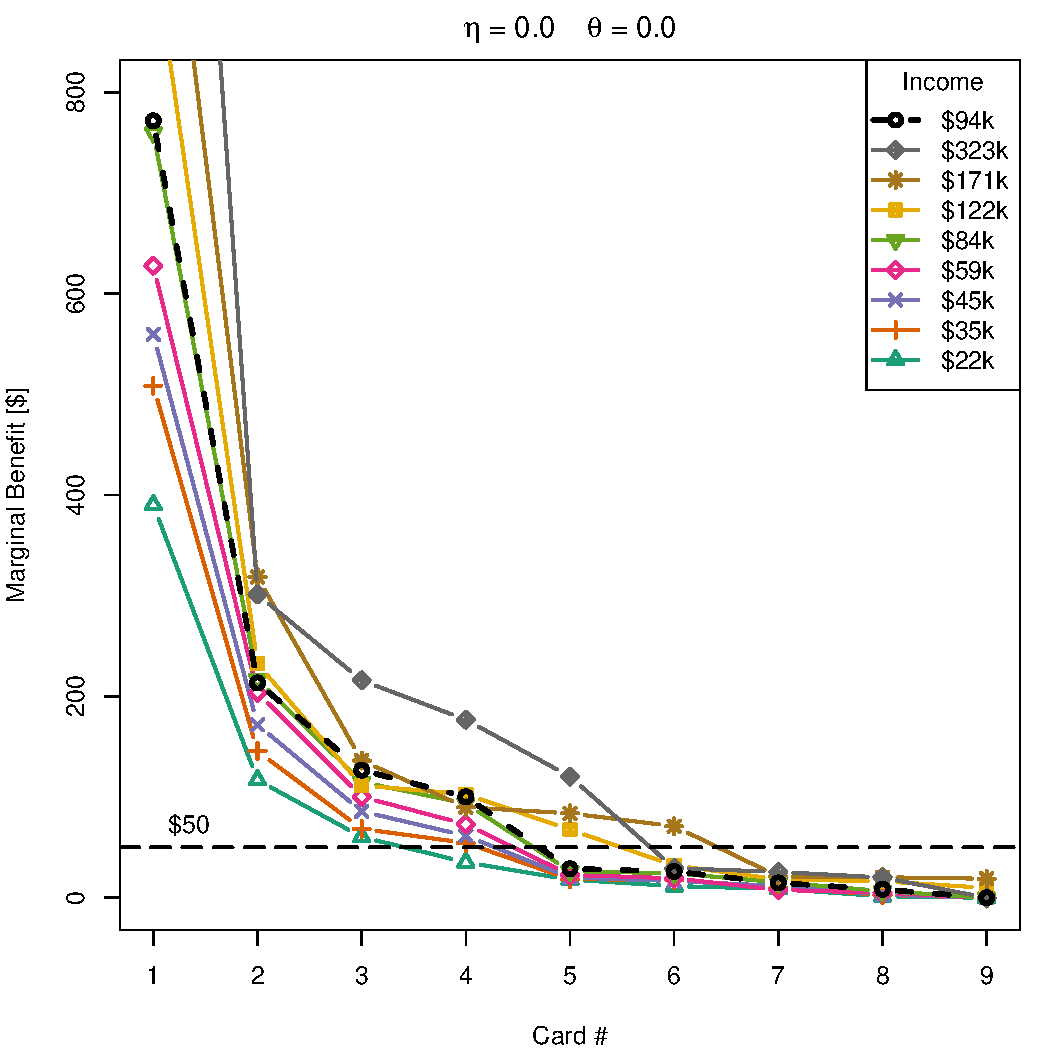
\includegraphics[width=0.6\textwidth]{../Figures/MBvsKvsIncome_0_0.pdf}
    \caption{Marginal benefit versus number of cards, assuming $(\eta, \theta) = (0,0)$.}
    \label{fig:MBvsKvsIncome_0_0}
    \end{center}
\end{figure}

\begin{figure}[tbh]
    \begin{center}
    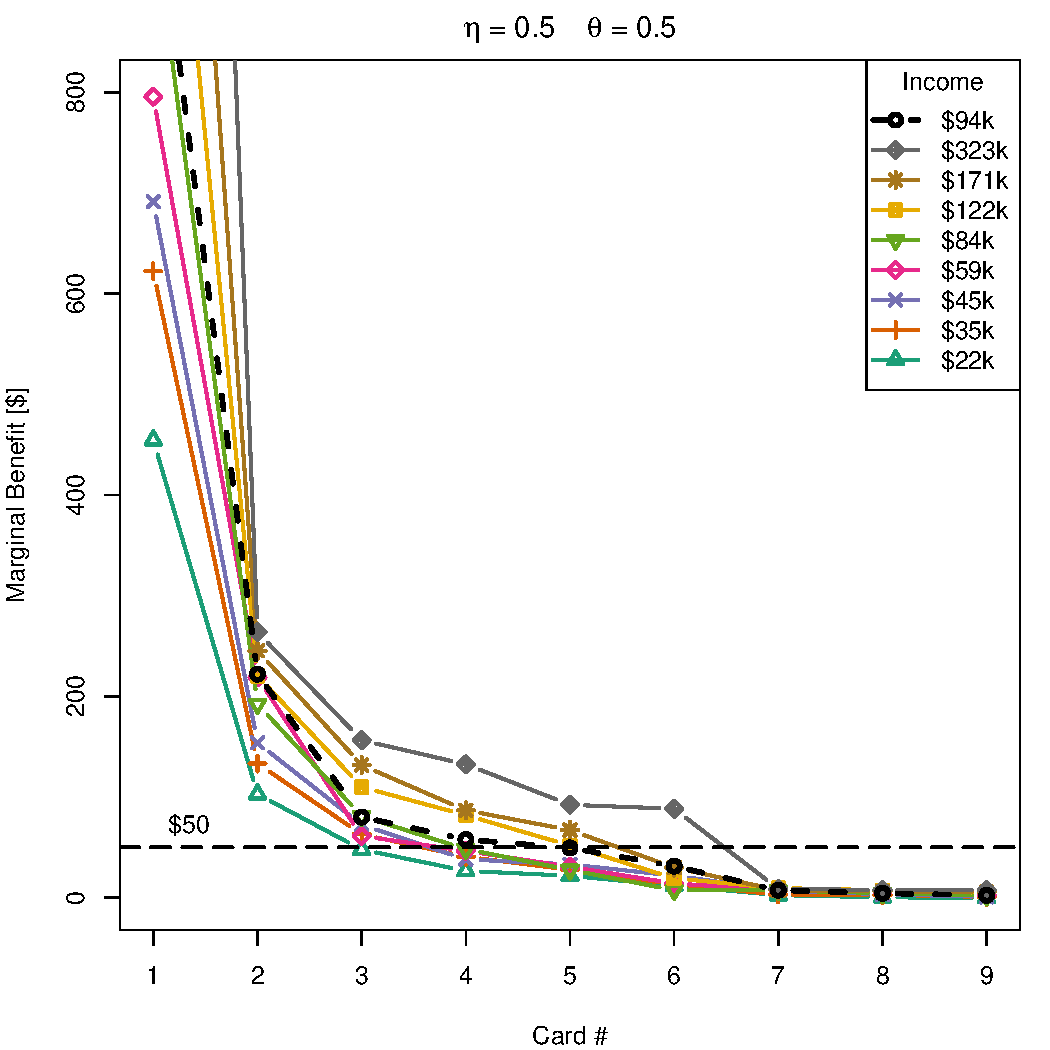
\includegraphics[width=0.6\textwidth]{../Figures/MBvsKvsIncome_05_05.pdf}
    \caption{Marginal benefit versus number of cards, assuming $(\eta, \theta) = (0.5,0.5)$.}
    \label{fig:MBvsKvsIncome_05_05}
    \end{center}
\end{figure}

\begin{figure}[tbh]
    \begin{center}
    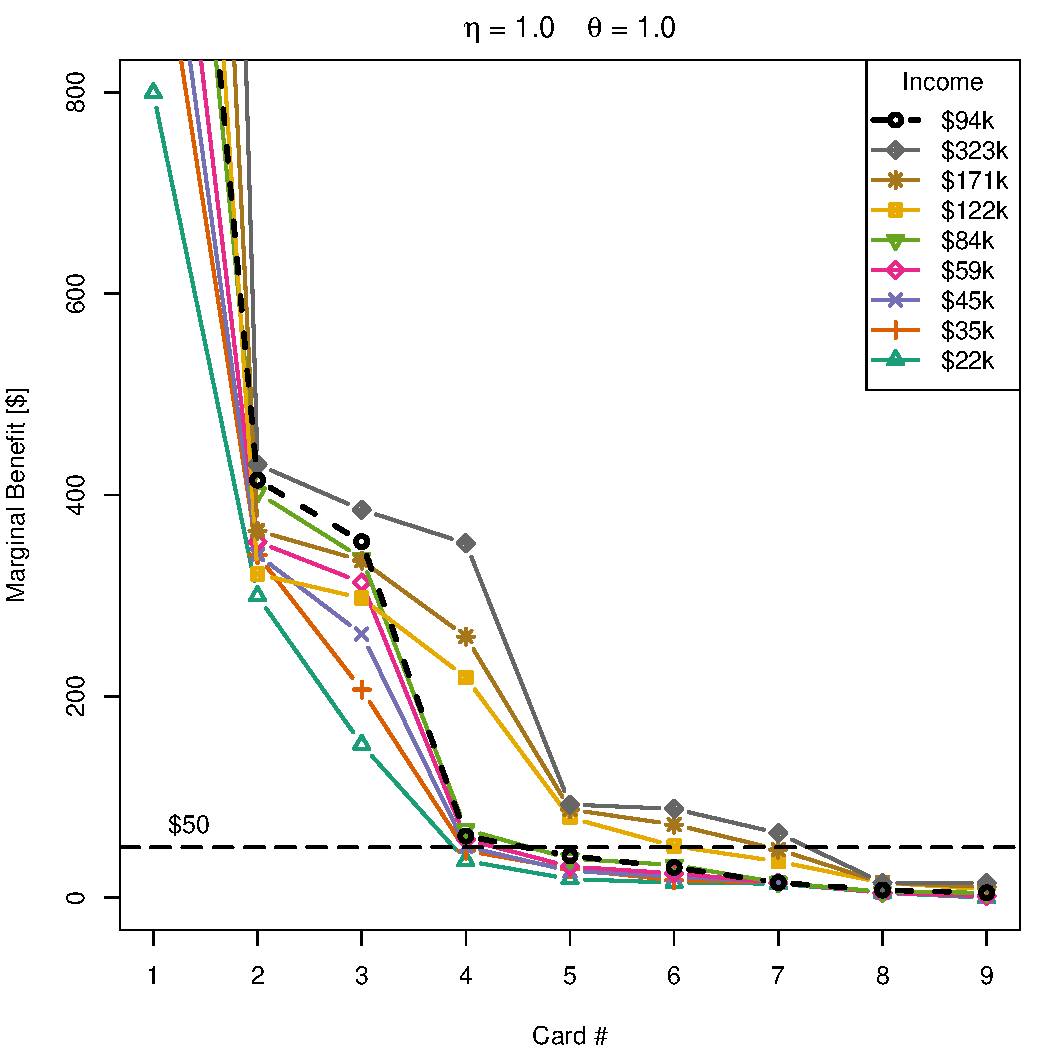
\includegraphics[width=0.6\textwidth]{../Figures/MBvsKvsIncome_1_1.pdf}
    \caption{Marginal benefit versus number of cards, assuming $(\eta, \theta) = (1,1)$.}
    \label{fig:MBvsKvsIncome_1_1}
    \end{center}
\end{figure}

\clearpage
Figures \ref{fig:ROSvsKvsIncome_0_0}, \ref{fig:ROSvsKvsIncome_05_05}, and \ref{fig:ROSvsKvsIncome_1_1} show the total return on spend versus the number of cards, for the same choice of $(\eta, \theta)$ as the previous three figures. 
These figures show that ROS converges to $\sim3.2$ percent for cashback-oriented users, regardless of income level (Fig.~\ref{fig:ROSvsKvsIncome_0_0}).
Once travel transfer partners and benefits are being used, Figs.~\ref{fig:ROSvsKvsIncome_05_05} and~\ref{fig:ROSvsKvsIncome_1_1} show that there is more variation among different income levels. 
As expected, travel and benefits return additional value, and increase ROS for all incomes.
Once all benefits are being used, however ($\theta = 1$, Fig.~\ref{fig:ROSvsKvsIncome_1_1}), we see an interesting reversal in the effect for different incomes: the lowest income levels reach a ROS comparable, or even higher, than the highest income levels (e.g., note the cyan triangles above the gray diamonds). 
Consumers at the lowest income levels can spend much less on credit cards compared to high-income consumers, but Fig.~\ref{fig:ROSvsKvsIncome_1_1} reminds us that low-income consumers can benefit more, relative to their spend, as long as they make full use of the static credit card benefits.
Figure~\ref{fig:ROSvsKvsIncome_1_1} also shows that 5.5--6.5 percent is roughly the maximum ROS people can expect, when making full use of an optimized portfolio of 4--5 credit cards.
 
\begin{figure}[tbh]
    \begin{center}
    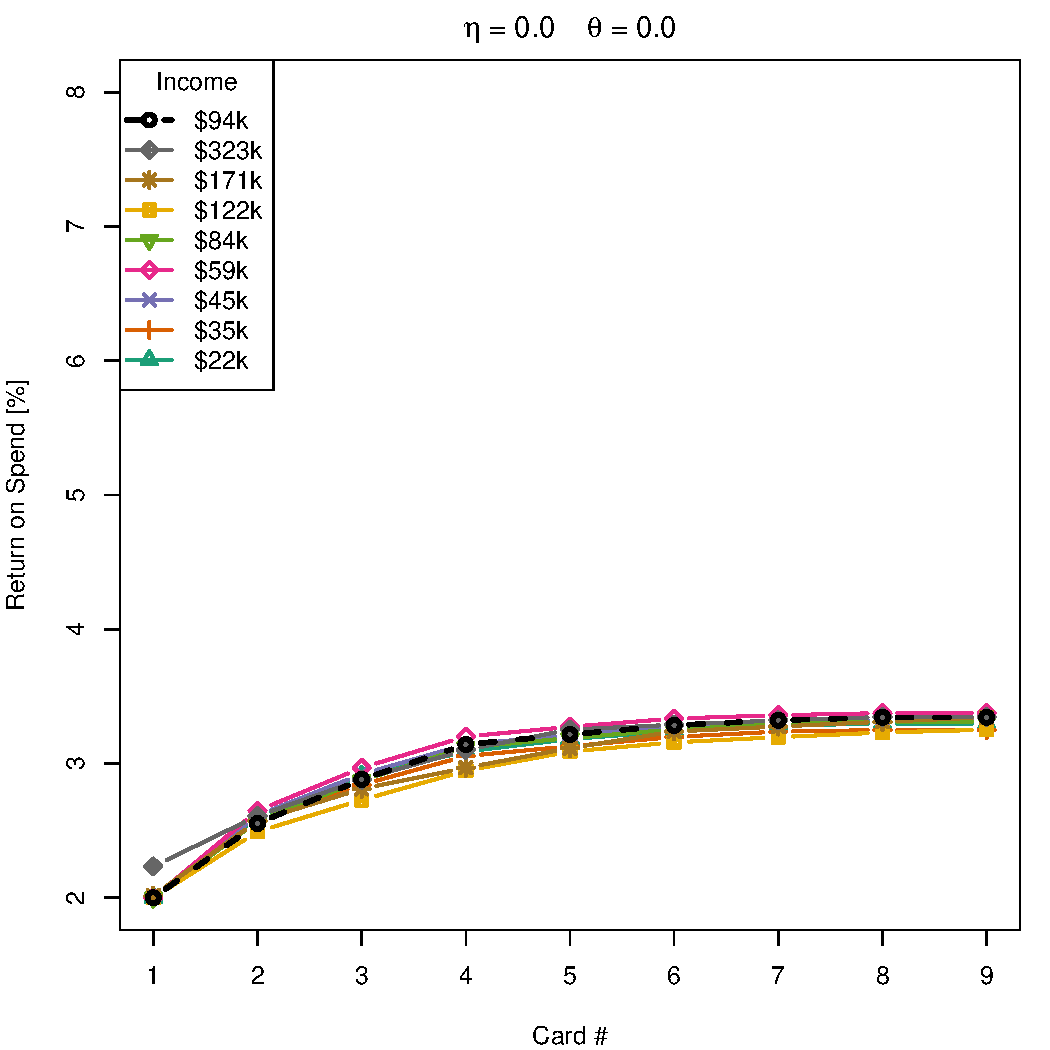
\includegraphics[width=0.6\textwidth]{../Figures/ROSvsKvsIncome_0_0.pdf}
    \caption{Total return on spend versus the number of cards, assuming $(\eta, \theta) = (0,0)$.}
    \label{fig:ROSvsKvsIncome_0_0}
    \end{center}
\end{figure}

\begin{figure}[tbh]
    \begin{center}
    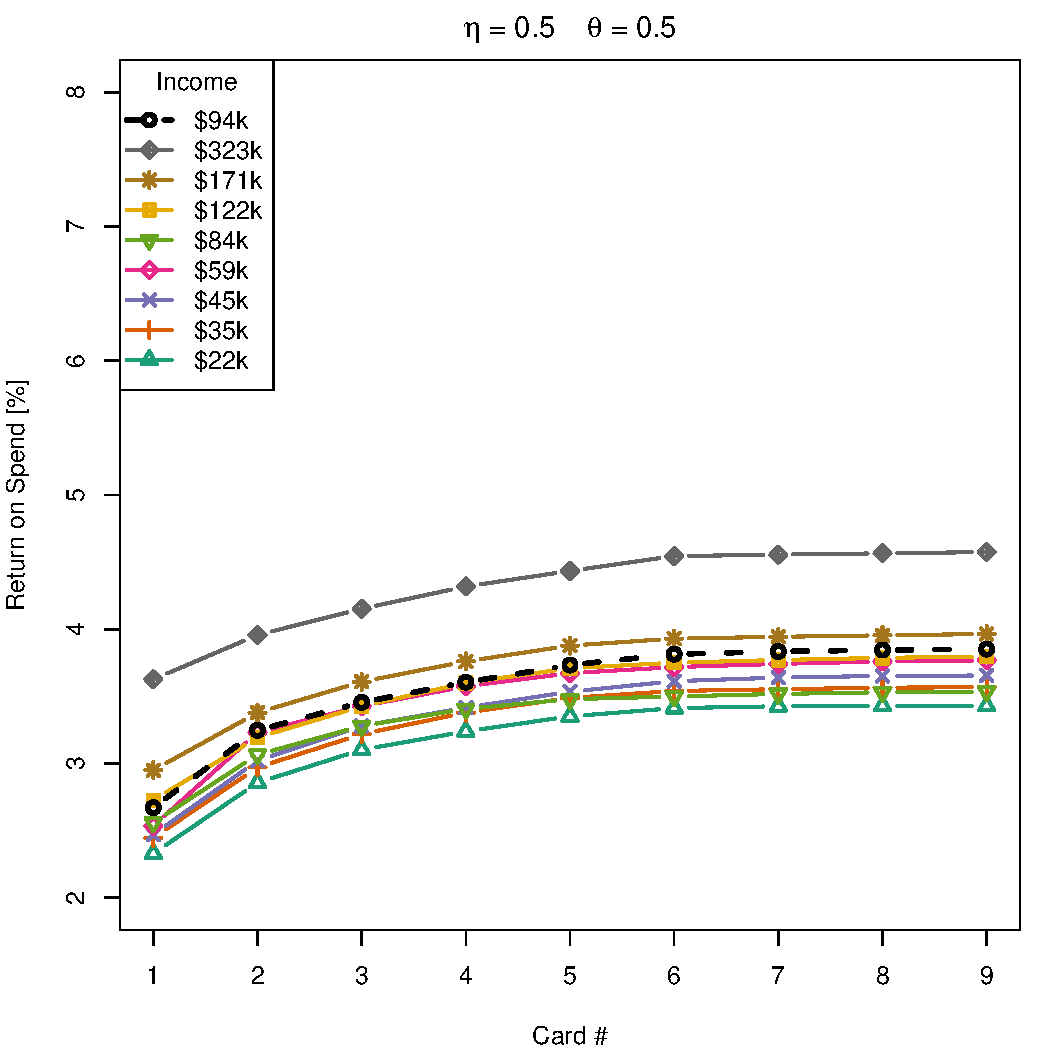
\includegraphics[width=0.6\textwidth]{../Figures/ROSvsKvsIncome_05_05.pdf}
    \caption{Total return on spend versus the number of cards, assuming $(\eta, \theta) = (0.5,0.5)$.}
    \label{fig:ROSvsKvsIncome_05_05}
    \end{center}
\end{figure}

\begin{figure}[tbh]
    \begin{center}
    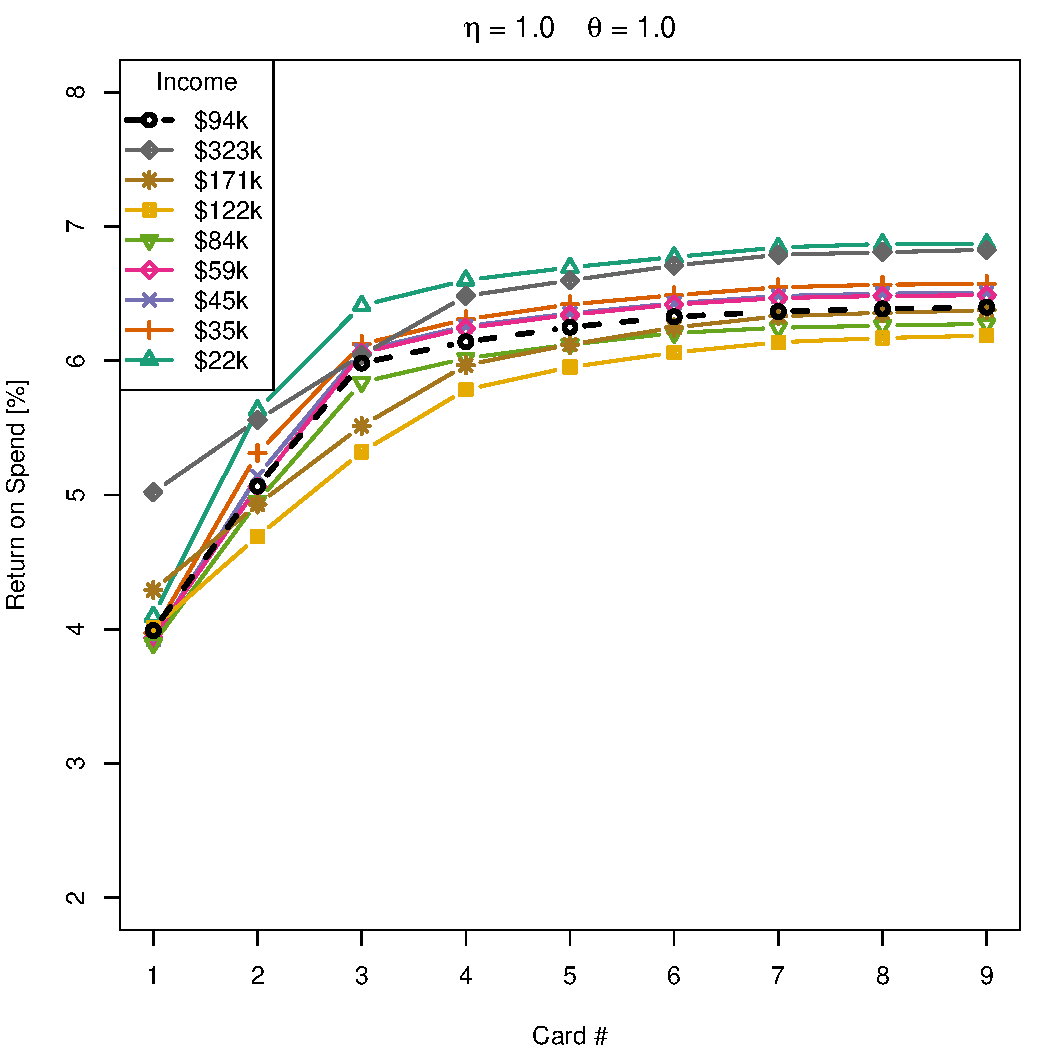
\includegraphics[width=0.6\textwidth]{../Figures/ROSvsKvsIncome_1_1.pdf}
    \caption{Total return on spend versus the number of cards, assuming $(\eta, \theta) = (1,1)$.}
    \label{fig:ROSvsKvsIncome_1_1}
    \end{center}
\end{figure}

\clearpage
Figure~\ref{fig:NBvsIncome} shows the range in total net benefit (in dollars) versus income.  
This range lies between $\sim\$700$--$\$1200$ for the lowest incomes, and increases all the way up to $\sim\$2000$--$\$5000$ for incomes above \$300k.

\begin{figure}[t!bh]
    \begin{center}
    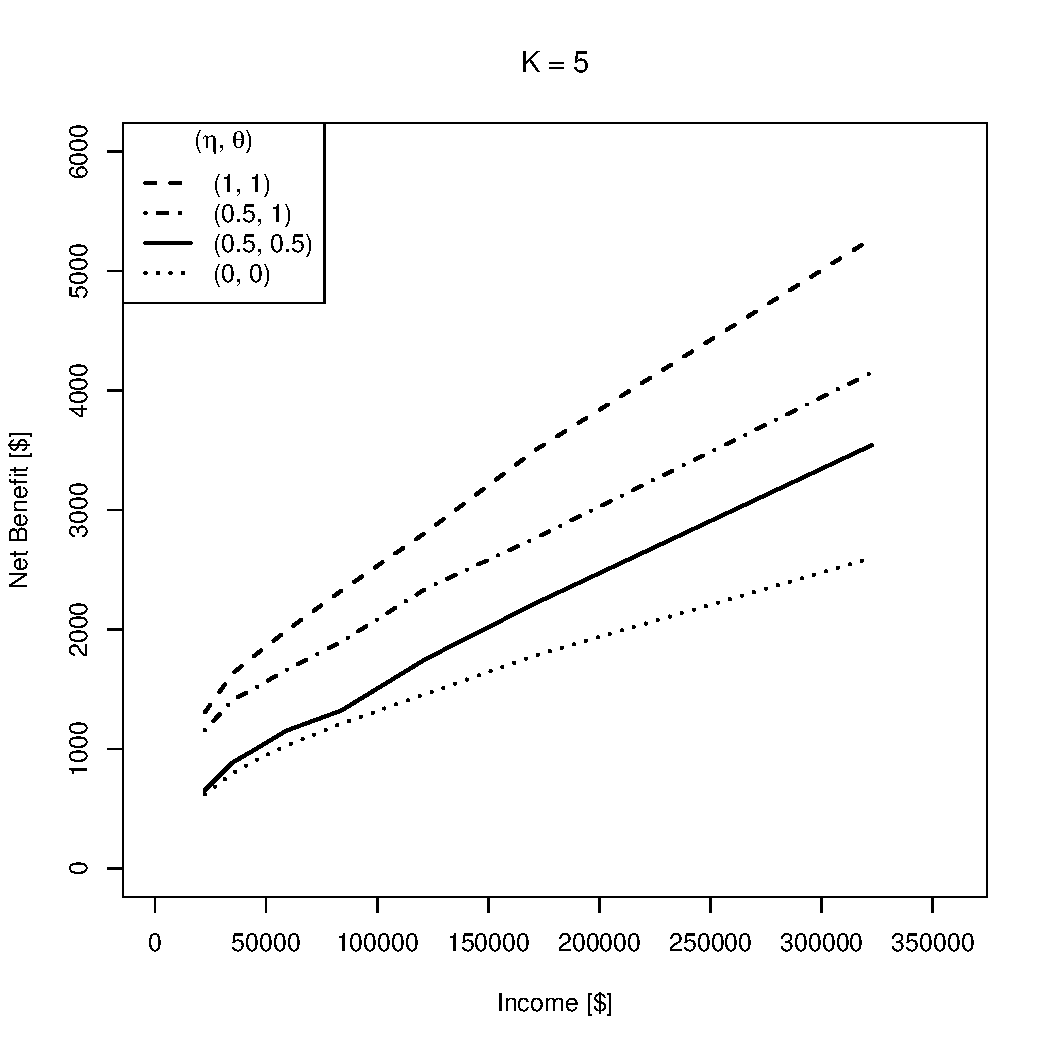
\includegraphics[width=0.6\textwidth]{../Figures/NBvsIncome_K5.pdf}
    \caption{The total net benefit versus income for different combinations of $\eta$ and $\theta$. }
    \label{fig:NBvsIncome}
    \end{center}
\end{figure}

\subsection{Monte Carlo Simulation}

Above we have seen how income and user preferences impact the expected return on spend from rewards credit cards.
Income affected these results in two ways, as can also be seen from Table~\ref{tab:BudgetIncome} in the Data Appendix.
First of all, total spend scales with income; people with higher incomes will spend more on credit cards, although the total spend as a fraction of income goes down (i.e., with increasing income, people put a fraction of the increase toward savings and housing, which does not end up on credit cards).
Second, with changing income there are also shifts in the spending budgets; essential goods like groceries and gas form a much larger part of the budget for lower incomes, compared to higher incomes. 

To represent more accurately how these patterns affect the benefits of rewards credit cards for a large group of users, I performed a Monte Carlo simulation using 100,000 samples. 
The family income distribution of 57,005 Floridians was used, as described in Sect.~\ref{sec:Data} and presented in Fig.~\ref{fig:IncomeDistribution}.
This distribution was sampled, with replacement, 100,000 times, and for each income the  average budget from the corresponding income bin from the BLS CES data was assumed. 
Each income was then combined with a random value for $K$ (between 1--8), $\eta$ (0--1), and $\theta$ (0--1), which were sampled from uniform distributions.
The optimal portfolio was determined for each sample, and results regarding net benefits, return on spend, and a count of each selected credit card was saved to a \texttt{.csv} file for further analysis. 
This simulation took roughly two hours to process on a 2023 MacBook Pro.

\begin{figure}[t!bh]
    \begin{center}
    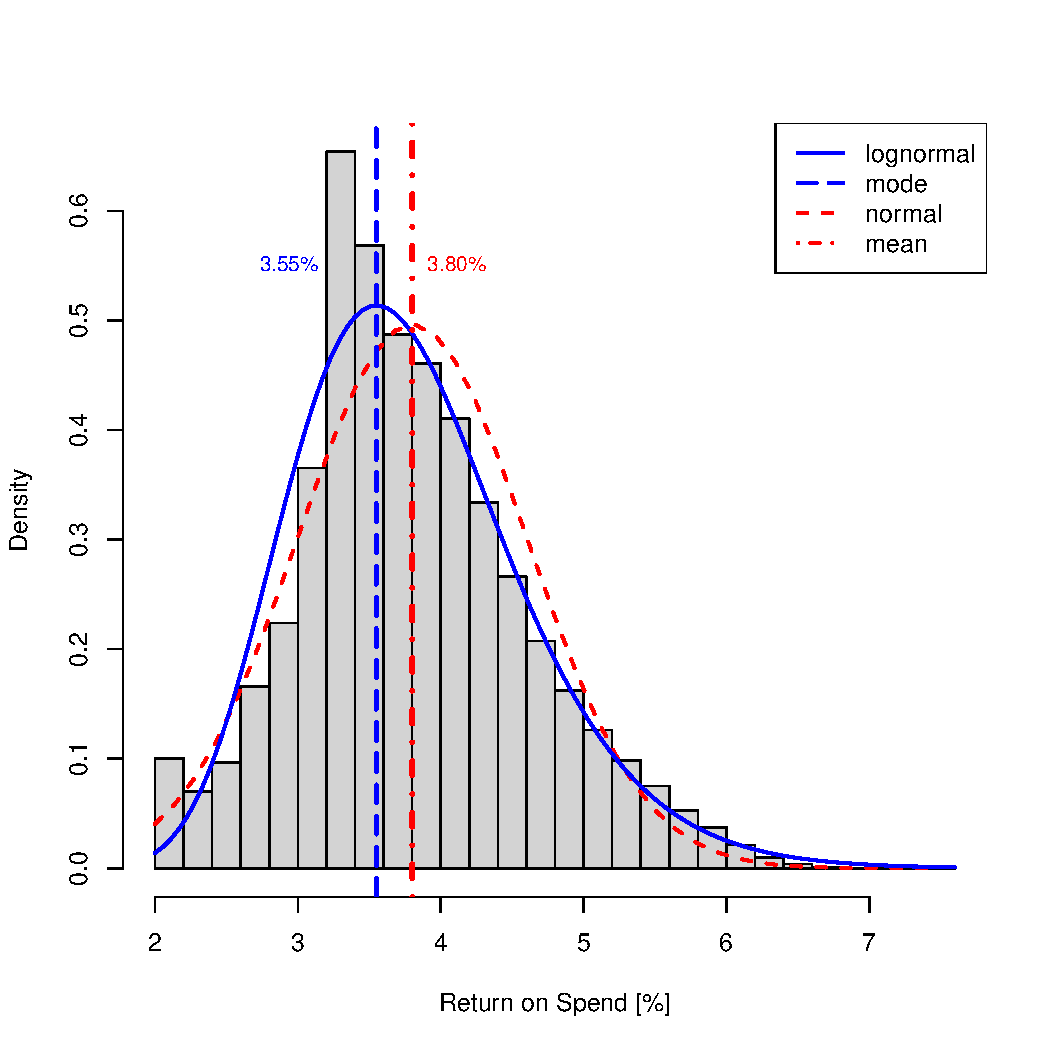
\includegraphics[width=0.6\textwidth]{../Figures/MC_ROS_Histogram.pdf}
    \caption{Distribution of return on spend, resulting from the Monte Carlo simulation.}
    \label{fig:MC_ROS_Histogram}
    \end{center}
\end{figure}

Figure~\ref{fig:MC_ROS_Histogram} shows the ROS distribution resulting from the Monte Carlo simulation.
The distribution approximates a lognormal with a mode at 3.55~percent, while the mean ROS is 3.80~percent with a standard deviation of 0.80.

\begin{figure}[t!bh]
    \begin{center}
    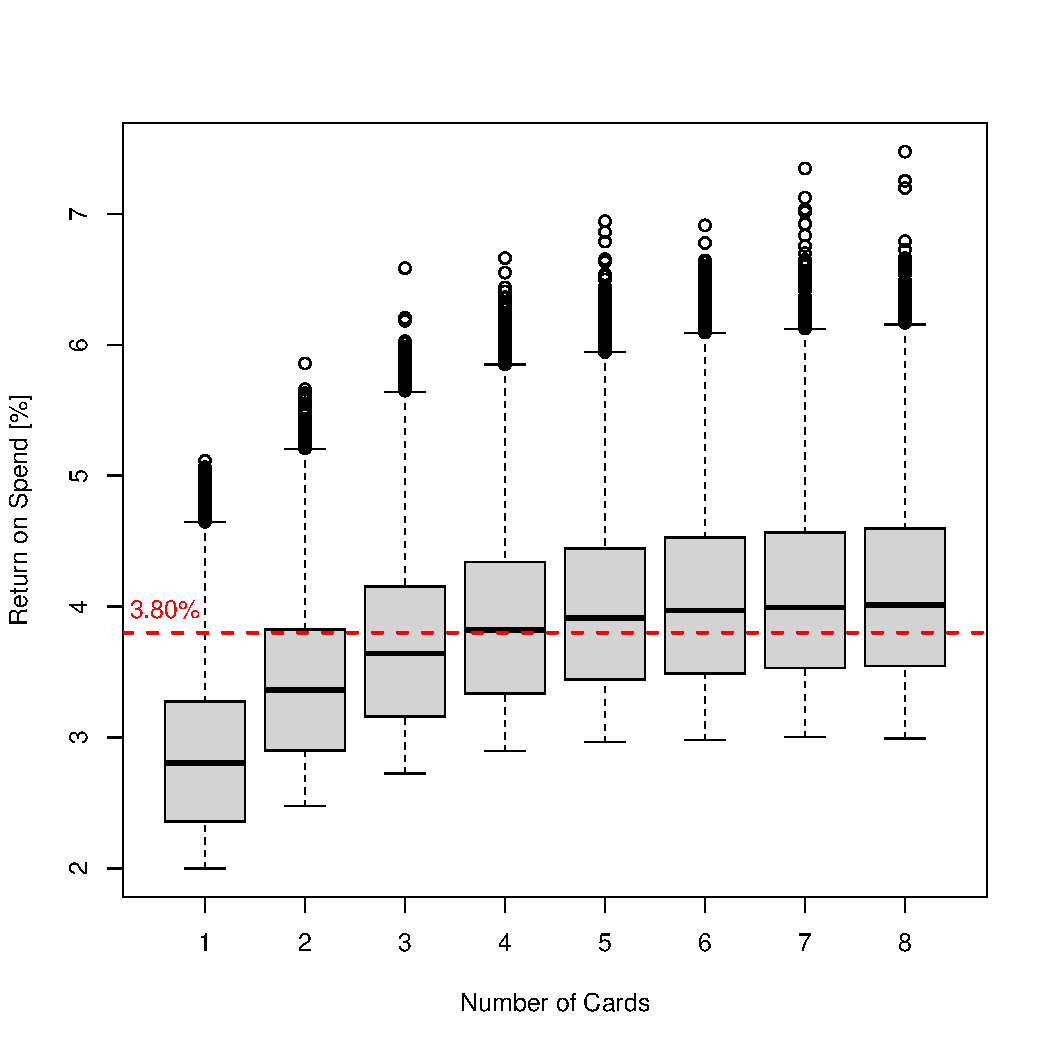
\includegraphics[width=0.6\textwidth]{../Figures/MC_ROS_vs_K.pdf}
    \caption{Boxplot of the return on spend versus the number of cards, resulting from the Monte Carlo simulation. The horizontal dashed line indicates the mean ROS of 3.80~percent, which is very close to the mean ROS of consumers using four credit cards.}
    \label{fig:MC_ROS_vs_K}
    \end{center}
\end{figure}

Figure~\ref{fig:MC_ROS_vs_K} shows a boxplot of the return on spend versus the number of cards, which confirms the earlier observations that marginal benefit diminishes strongly after four or five cards.

Using a logarithmic scale for income, Fig.~\ref{fig:MC_ROS_vs_Income} shows a smoothed density scatterplot of all 100,000 simulated portfolios.  
This shows where the highest density of our ``observations'' are, as well as how ROS varies with income. 
Per income, the vertical spread in density is caused by the random sampling of $K$ (number of cards), $\eta$ (use of transfer partners), and $\theta$ (use of benefits).
The spread in the horizontal direction is caused by the observed Floridian income distribution.
A ``loess'' curve (short for ``locally estimated scatterplot smoothing'') is overplotted in red, and highlights a trend where the mean ROS is increasing for incomes above $\sim\$120,000$.
This upward trend must be attributed to shifts in spending patterns with income. 
Looking at the fraction of spend going toward the travel, dining, and groceries categories in Fig.~\ref{fig:TravelDiningFraction}, we see that essentials like groceries becomes a less important part of the budget as income increases.
Travel, on the other hand, takes up a larger fraction of the budget for higher incomes, while dining (away from home) shows this effect to a smaller degree. 
Not surprisingly, in our credit cards dataset we find some of the highest point multipliers on the travel categories, usually on cards with the highest annual fees, such as the American Express Platinum and the Chase Sapphire Reserve. 
High-income individuals can more easily justify these high annual fees, especially since they also have the spending behavior that matches well with the rewards categories of these cards, leading to above-average benefits.   

\begin{figure}[t!h]
    \begin{center}
    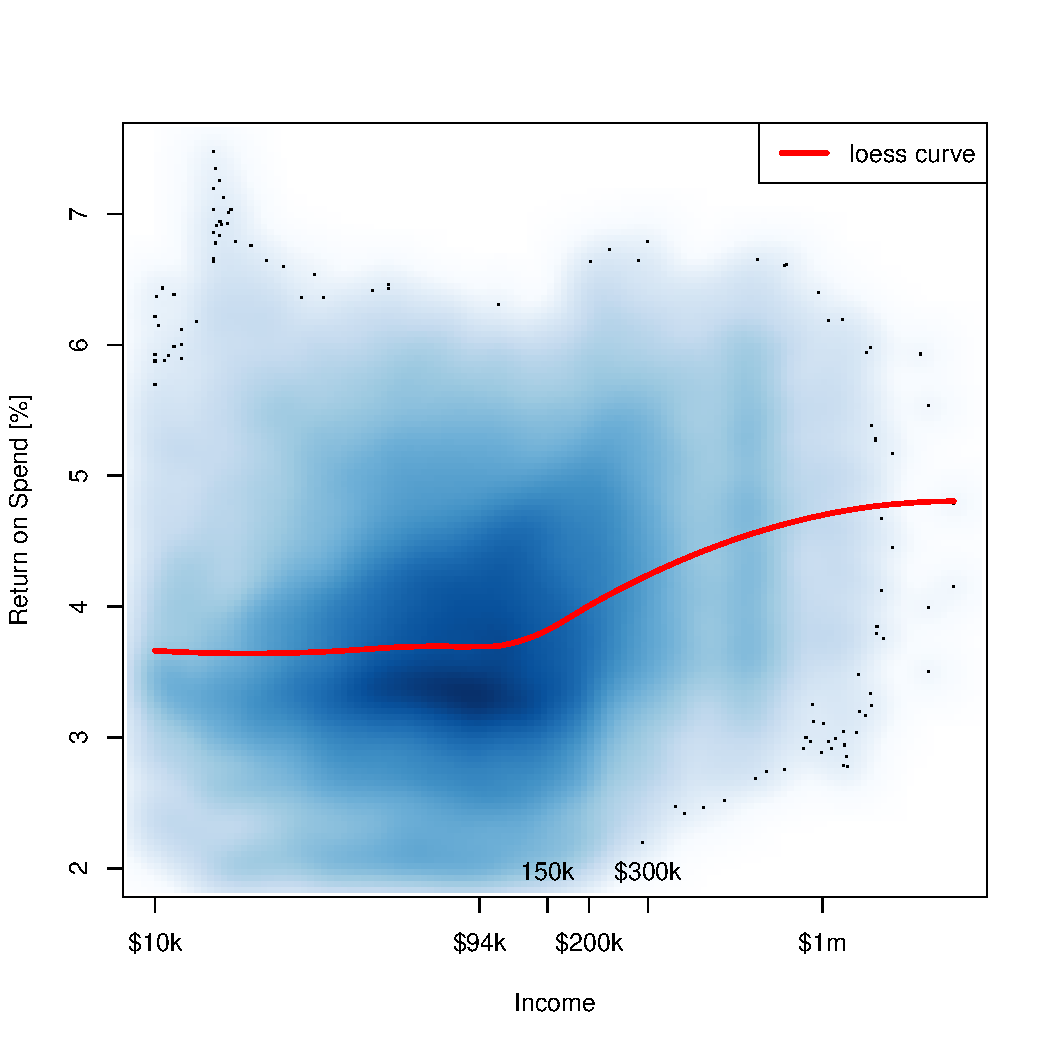
\includegraphics[width=0.6\textwidth]{../Figures/MC_ROS_vs_Income.pdf}
    \caption{Smoothed density scatterplot of return on spend versus income, for all 100,000 simulated portfolios.}
    \label{fig:MC_ROS_vs_Income}
    \end{center}
\end{figure}

\begin{figure}[t!h]
    \begin{center}
    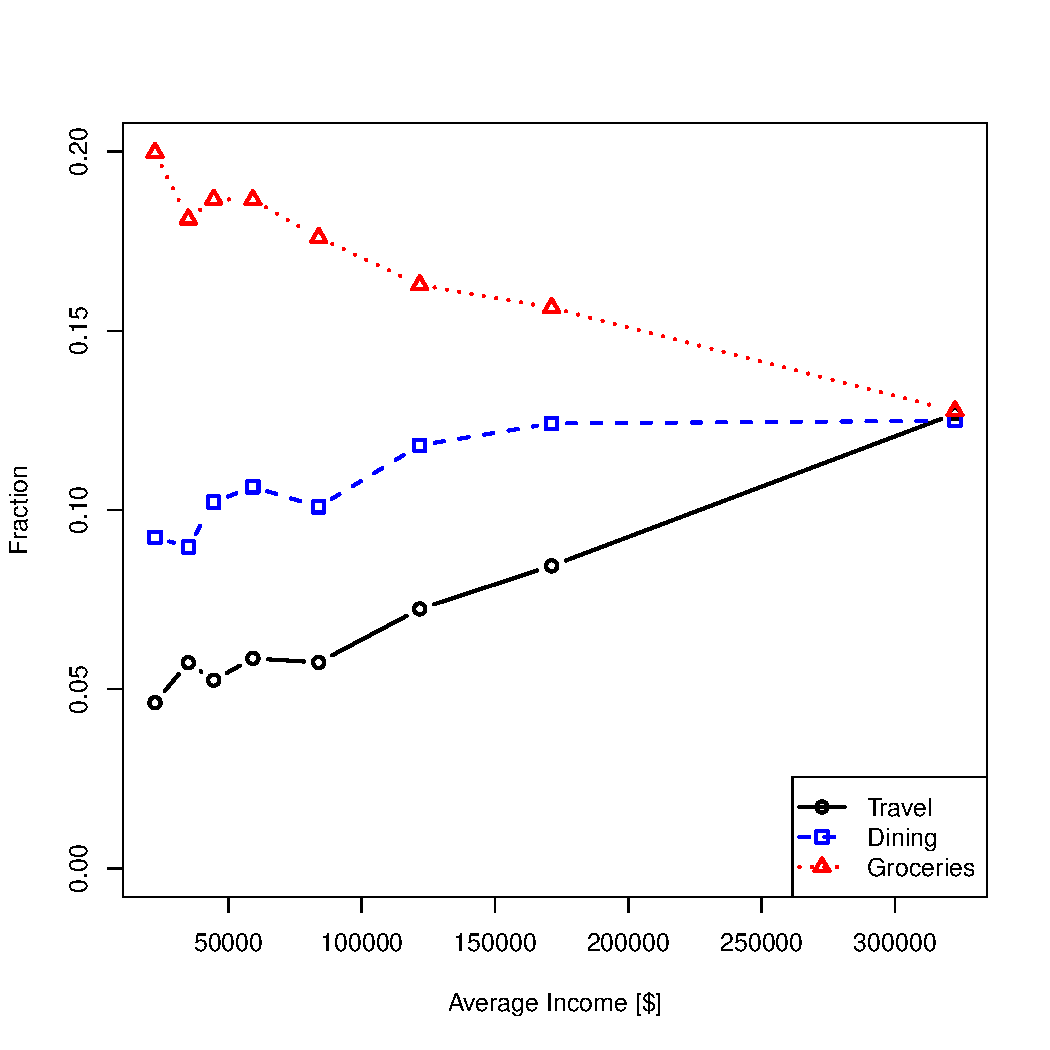
\includegraphics[width=0.6\textwidth]{../Figures/TravelDiningFraction.pdf}
    \caption{Fraction of total credit card spend going toward travel, dining, and groceries, for the average incomes from the BLS CES data (mapped to the credit card spending categories).}
    \label{fig:TravelDiningFraction}
    \end{center}
\end{figure}

Finally, the results of the Monte Carlo simulation can be used to show how often a specific credit card ends up in a recommended portfolio. 
Figure~\ref{fig:MC_Popularity_100k} shows the top 10 most recommended cards. 
The Amazon Prime card and the American Express Blue Cash Preferred are the two most recommended cards, followed closely by the Wells Fargo Autograph.

\begin{figure}[t!bh]
    \begin{center}
    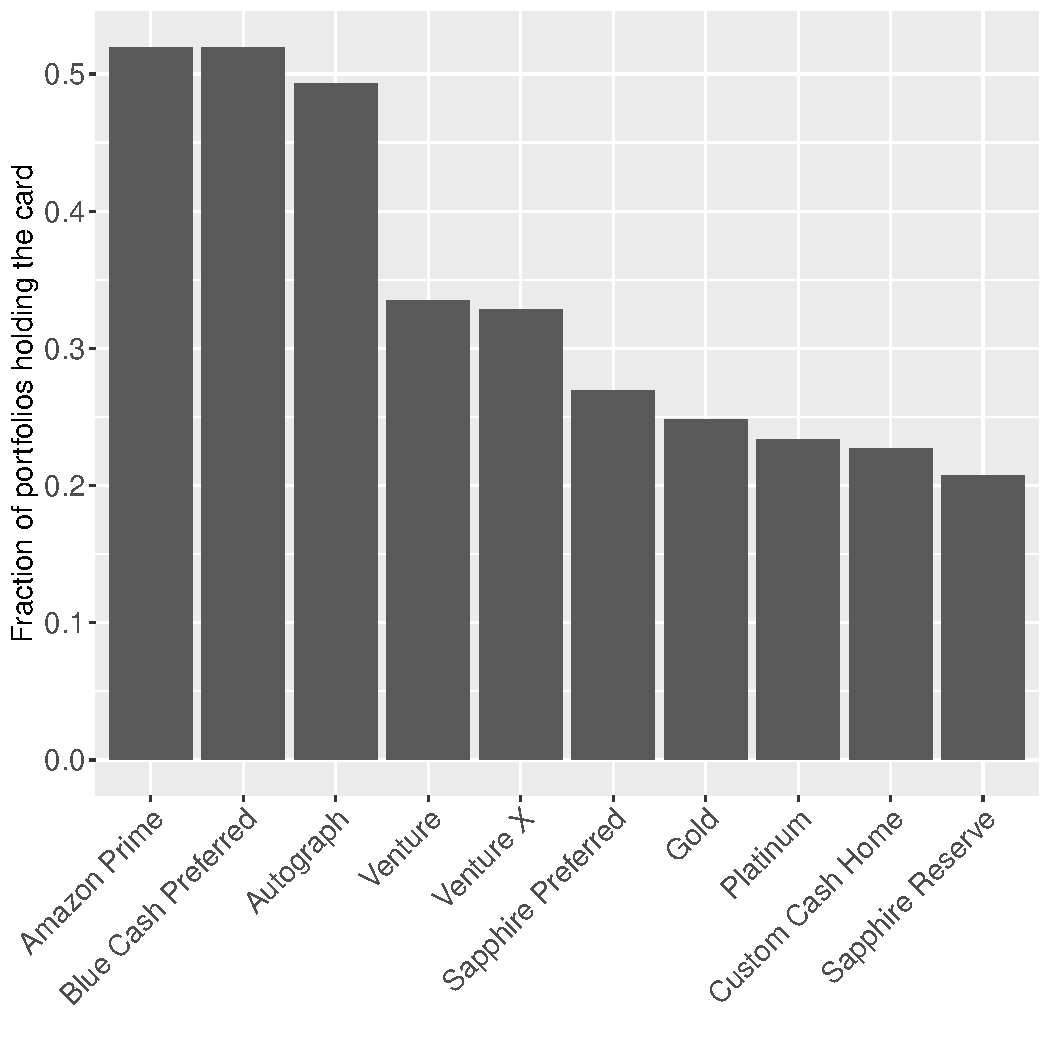
\includegraphics[width=0.6\textwidth]{../Figures/MC_Popularity_M100k.pdf}
    \caption{Top 10 most recommended credit cards from the Monte Carlo simulation.}
    \label{fig:MC_Popularity_100k}
    \end{center}
\end{figure}

\clearpage
\subsection{Shiny App} \label{subsec:ShinyApp}

No credit card user is the same. 
Above we have seen how credit card rewards can benefit users with average income levels and average budgets, but what we really need is a way to make \emph{personal} recommendations based on someones individual spending behavior, point valuations, and other preferences. 
This is why I have also developed an \sR\ \textsf{Shiny} app that will return the optimal portfolio for a user's personal preferences and individual budget.

A screenshot of the current version of the app is shown in Fig.~\ref{fig:REMCCO}, and the app can be accessed online at \url{https://remcoscheepmaker.shinyapps.io/ReMCCO/}.%
\footnote{The working title of the app is ``ReMCCO,'' which stands for Recommend Me Credit Cards Optimally.}
Every \textsf{Shiny} app consists of a user interface and a server function. 
The server function makes use of exactly the same \texttt{get\_budget()} and \texttt{get\_portfolio()} functions as the rest of this project (presented in the Code Appendix), so the underlying algorithm works the same (although the app rounds the budget to the nearest dollar, which explains small differences between Figs.~\ref{fig:Waterfall} and \ref{fig:REMCCO}).

In the left column of the user interface, a user can specify preferences such as number of cards ($K$), use of transfer partners ($\eta$), use of benefits ($\theta$), and which banks to include. 
In a second column, the spending budget is pre-filled to match an average budget based on income (using Table~\ref{tab:BudgetIncome}), but the user can adjust this budget freely, either by adjusting the income, or by changing the amount for each category individually, making the budget completely personal. 
The waterfall plot in the top right will automatically adjust after each change (using \textsf{Shiny's} ``reactive'' programming functionality). 
This waterfall plot shows the recommended credit card portfolio, including the marginal and total benefits, just like Fig.~\ref{fig:Waterfall}. 
Underneath the figure some summary information is printed, and the card assignments are presented in a table (to show which card to use for each spending category).

In its current form, the app already has more functionality than what was captured by the variables and parameters that I used in the analysis above, since the user can also filter for banks and personalize the budget. 
The app could be further improved, however, by also making the valuations of points and benefits user-adjustable. 
This way, the user can specify that it values points or benefits from certain banks differently, for example because one bank has a transfer partner that the user really values, or because the user is a preferred client at one bank, which might come with additional benefits.%
\footnote{For example, Bank of America's \emph{Preferred Rewards} program offers 25, 50, or 75~percent higher point values for clients with \$20,000, \$50,000, or \$100,000 in combined assets at Bank of America / Merrill.} 
A future update of the app is planned to include these improvements. 

\begin{landscape}
\begin{figure}[t!h]
    \begin{center}
    \includegraphics[scale=0.45]{../Misc/REMCCO.png}
    \caption{Screenshot of the online \sR\ \textsf{Shiny} user interface at \url{https://remcoscheepmaker.shinyapps.io/ReMCCO/}.}
    \label{fig:REMCCO}
    \end{center}
\end{figure}
\end{landscape}


% \section{Conclusions} \label{sec:Conclusions}

We have seen that credit cards can be very rewarding for those (financially sophisticated) people who have the discipline to pay them off in full each month.
Due to inefficiencies in the the rewards programs, it is mostly people who use cash, or the (financially na\"{i}ve) people who use credit cards in a nonoptimal way, who are paying for the rewards of the financially sophisticated, through inflated prices, interest, and fees. 
Also the people who use credit cards optimally, however, pay for some fraction of their rewards through the same inflated prices, that merchants most likely have raised to recoup some of the interchange fees set by the credit card networks.

By developing a credit card recommendation algorithm, I have shown that people can expect an ROS of up to $\sim$6.5~percent, by putting all their spend on up to 4--6 credit cards.
A Monte Carlo simulation showed that the mean expected ROS is $3.80\pm0.80$~percent, and 
the ROS is higher for people who are using travel transfer partners for their points, and who make use of all the static benefits that credit cards might offer.
These numbers assume that people are willing to put in some time and research into their personal finances, in order to estimate their yearly spending patterns and apply for those cards that best fit this spending budget. 
To help with this, I have developed an online app that takes a user's budget and preferences into account, in order to recommend the optimal credit card portfolio.

My results also show a trend of ROS increasing with income, once a threshold income of roughly \$120,000 is reached. 
This is most likely explained by a shift in spending patterns, as people with higher incomes spend an increasing fraction of their budget on travel, which is a category that offers higher rewards, without any meaningful spending limits (caps). 
Categories like groceries, or custom categories with elevated 5x multipliers, on the other hand, usually come with caps on the amount of rewards that can be earned, limiting the ROS on these categories for big spenders with high incomes.
The observation that ROS increases with income seems consistent with the conclusion from \cite{agaretal:2023} that reward credit cards are widening existing disparities between the poor and the rich.
% mention that this fits in the picture where banks stimulate overspending and affluent lifestyles? 

Since this project was planned, executed, and presented in a total timespan of about 11 weeks, I had to ignore certain details, and make some reasonable assumptions. 
For example, I have ignored foreign transaction fees, which are typically 3~percent for non-travel oriented credit cards. 
Travel credit cards usually do not have foreign transaction fees, but this still means that frequent international travelers have to leave certain other cards from their portfolio at home, complicating the optimal portfolio.
With 119 million merchants accepting American Express internationally, compared to 130 million accepting Visa/Mastercard \citep{thriftytraveler:2024}, the acceptance rate for American Express is still significantly lower abroad. 
This might also complicate someone's decision to choose credit cards, and is part of the reason why I included a bank filter in the \textsf{Shiny} app. 

One of the assumptions I made is that all users qualify for all the cards in the dataset, because I assumed that users are financially sophisticated, with high FICO scores, before they even want to optimize their credit card portfolio.  
One could argue indeed that this is not very realistic, and even with a prime-plus or super-prime credit score (i.e., a FICO score above 720, see Table~\ref{tab:FICO} on page~\pageref{tab:FICO}), the income of a user might not be high enough to get approved for certain cards that come with high credit lines. 
Banks, however, do not openly share their income and credit score requirements for their credit cards, and they probably also use other, non-disclosed, information to make approval decisions. 
So, even if a user would be asked to provide their income and FICO score in the app, 
an algorithm could only guess for which cards the user would be approved. 
Due to the time constraints, I have not included such an approval estimate in my algorithm, but it is feature to consider for a future update.
Until then, users of the app should understand that the recommended portfolio is something to aim for, even if certain cards seem currently unfeasible, based on the user's current income and credit score. 

Despite all these assumptions, I hope my app delivered some utility to the reader and my fellow classmates, and that this project has led to an increased awareness, and understanding, of the economics of credit card rewards, and the benefits for their financially sophisticated users. 


% \section*{Acknowledgements}

% This capstone project would not have been possible without Dr.~Harry Paarsch. 
I would like to thank him for all his teachings and guidance throughout the last year, and for his book with Dr.~Konstantin Golyaev \citep{paargoly:2016}.
He made me realize that economics is much closer to a real (natural) science than I always feared. 
I would also like to thank all the other professors that made this first cohort of the Business Analytics program possible: Dr.~Lealand Morin, Dr.~Alexander Mantzaris, and Dr.~Majid Mahzoon for their software and data visualization classes. 
Dr.~Michael Tseng for his math class and Dr.~Nizam Uddin for his class on probability and statistics. 
I thank Dr.~Morgan Wang for introducing me to SAS, and I would like to thank Mr.~Joshua Eubanks for teaching me my first microeconomics class.
I would also like to thank Ms.~Meredith Smart for enrolling me exactly on schedule, every Friday before the start of the semester.

Finally, I would like to thank my fellow Business Analytics students from the 2023--2024 cohort, who made going back to school after 15 years a lot more fun. 
Malak, Kelly, Cody, Jared, Manoj, Nili, Frank, Danielle, Yasmeen, Anabella, and Avery: thanks for all the discussions, and for putting up with me and my Dutch directness. 
I'm wishing you all the best in your future careers, wherever those may bring you. 
Go Knights, and stay curious! 


% \section*{A. Appendix}

% In this appendix,


\singlespacing

\bibliographystyle{../chicago}
%\bibliographystyle{plainnat}
\bibliography{../References}
% The final section of the outline should include the list of readings.
% The list of readings should be single-spaced with one blank line between references, and generated using the reference management software BIBTEX. 

% The outline should not exceed twelve pages in length.
\end{document}
